\documentclass{article}




\usepackage{fullpage}
\usepackage{nopageno}
\usepackage{amsmath}
\usepackage{amsfonts}
\usepackage{graphicx}
\usepackage{framed}
\usepackage{algorithmic}
\usepackage{xcolor}

\definecolor{dark_red}{rgb}{0.5,0.0,0.0}
\definecolor{dark_green}{rgb}{0.0,0.5,0.0}
\definecolor{dark_blue}{rgb}{0.0,0.0,0.5}
\definecolor{blue}{rgb}{0.0,0.0,1.0}

\newcommand{\dr}[1]{\textcolor{dark_red}{#1}}
\newcommand{\dg}[1]{\textcolor{dark_green}{#1}}
\newcommand{\db}[1]{\textcolor{dark_blue}{#1}}
\newcommand{\blue}[1]{\textcolor{blue}{#1}}


\usepackage{fancyhdr}
%\setlength{\footheight}{15.2pt}
\pagestyle{fancy}
\fancyhead[C]{Wentworth Institute of Technology, MATH2025}
\fancyfoot[C]{Author: Shawn Eastwood}
\renewcommand{\headsep}{25pt}
\renewcommand{\headrulewidth}{1pt}
\renewcommand{\footrulewidth}{1pt}


\begin{document}

\section*{Introduction to vectors}

A {\bf vector} is an ordered list of numbers. The length of the list is a positive integer, and the order of the entries matters. A vector is commonly denoted by listing the entries in triangular braces:
\[\langle u_1, u_2, u_3, ..., u_n \rangle\]
or, by listing the entries from top to bottom:
\[\begin{bmatrix} u_1 \\ u_2 \\ u_3 \\ \vdots \\ u_n \end{bmatrix}\]

In contrast, a {\bf scalar} is a single number.

Variables that are vectors are often denoted by using boldface letters such as \(\mathbf{u}, \mathbf{v}, \mathbf{w}, ...\) in print, but in handwriting, vectors are often denoted by placing a left-to-right arrow above the chosen symbol: \(\vec{u}, \vec{v}, \vec{w}, ...\).

%\textbf{Examples:}
%\begin{itemize}
%\item A list of bank account balances.
%\item A list of 
%\end{itemize}

The symbol \(\mathbb{R}\) denotes the set of real numbers. The set of all vectors that have a length of \(n\) will be denoted by \(\mathbb{R}^n\). 

A common convention that will be used is that if a vector variable is denoted via a boldface letter, such as \(\mathbf{u}\), then the entries of the vector will be denoted using the same letter, but not in boldface, and using subscripts that start at \(1\) and count up to the length of the vector:

\[\mathbf{u} = \begin{bmatrix} u_1 \\ u_2 \\ u_3 \\ \vdots \\ u_n \end{bmatrix} \in \mathbb{R}^n\] %\mathbb{R} \times \mathbb{R} \times \mathbb{R} \times \cdots \times \mathbb{R} = \mathbb{R}^n\]

The ``zero vector", denoted by \(\mathbf{0}\), is a vector where every entry is \(0\). There is a different zero vector for each possible number of entries, and the number of entries in the zero vector \(\mathbf{0}\) depends on context. 




\subsection*{Basic vector arithmetic}

Now will be described the most basic of vector arithmetic, addition and scalar multiplication. Given two arbitrary vectors that have the {\bf same number of entries}, 
\[\mathbf{u} = \begin{bmatrix} u_1 \\ u_2 \\ u_3 \\ \vdots \\ u_n \end{bmatrix} \quad\text{and}\quad \mathbf{v} = \begin{bmatrix} v_1 \\ v_2 \\ v_3 \\ \vdots \\ v_n \end{bmatrix}\]

the vector sum is derived by simply adding together the corresponding entries:
\[\mathbf{u} + \mathbf{v} = \begin{bmatrix} u_1 \\ u_2 \\ u_3 \\ \vdots \\ u_n \end{bmatrix} + \begin{bmatrix} v_1 \\ v_2 \\ v_3 \\ \vdots \\ v_n \end{bmatrix} = \begin{bmatrix} u_1 + v_1 \\ u_2 + v_2 \\ u_3 + v_3 \\ \vdots \\ u_n + v_n \end{bmatrix}\]

\textbf{Examples:}
\begin{itemize}
\item 
\[\begin{bmatrix} 4 \\ -5 \end{bmatrix} + \begin{bmatrix} 13 \\ 7 \end{bmatrix} = \begin{bmatrix} 4 + 13 \\ -5 + 7 \end{bmatrix} = \begin{bmatrix} 17 \\ 2 \end{bmatrix}\]
\item 
\[\begin{bmatrix} 41 \\ -23 \\ 95 \end{bmatrix} + \begin{bmatrix} -27 \\ 70 \\ -113 \end{bmatrix} = \begin{bmatrix} 41 + (-27) \\ -23 + 70 \\ 95 + (-113) \end{bmatrix} = \begin{bmatrix} 14 \\ 47 \\ -18 \end{bmatrix}\]
\item 
\[\begin{bmatrix} -7 \\ 12 \end{bmatrix} + \begin{bmatrix} 16 \\ 10 \\ -8 \end{bmatrix} = \text{undefined}\]
\end{itemize}

Next, {\bf scalar multiplication} involves the multiplication of a vector by a single scalar (single number). To motivate scalar multiplication, consider the following:

Let \(k\) denote an arbitrary natural number, and let \(x\) denote an arbitrary real number. By the very definition of multiplication, \(k \cdot x\) is the sum involving \(k\) copies of \(x\): 
\[k \cdot x = \underbrace{x + x + ... + x}_k\]

Let \(\mathbf{u} = \begin{bmatrix} u_1 \\ u_2 \\ u_3 \\ \vdots \\ u_n \end{bmatrix}\) denote an arbitrary \(n\) component vector. Analogous to the multiplication of scalars, \(k \cdot \mathbf{u}\) is the sum involving \(k\) copies of \(\mathbf{u}\):
\[k \cdot \mathbf{u} = \underbrace{\mathbf{u} + \mathbf{u} + ... + \mathbf{u}}_k = \underbrace{\begin{bmatrix} u_1 \\ u_2 \\ u_3 \\ \vdots \\ u_n \end{bmatrix} + \begin{bmatrix} u_1 \\ u_2 \\ u_3 \\ \vdots \\ u_n \end{bmatrix} + ... + \begin{bmatrix} u_1 \\ u_2 \\ u_3 \\ \vdots \\ u_n \end{bmatrix}}_k = \begin{bmatrix} k \cdot u_1 \\ k \cdot u_2 \\ k \cdot u_3 \\ \vdots \\ k \cdot u_n \end{bmatrix}\]

More generally, if \(c\) is an arbitrary scalar, then:

\[c\mathbf{u} = \mathbf{u} c = c\begin{bmatrix} u_1 \\ u_2 \\ u_3 \\ \vdots \\ u_n \end{bmatrix} = \begin{bmatrix} c u_1  \\ c u_2 \\ c u_3 \\ \vdots \\ c u_n \end{bmatrix}\]

In the same vein, the ``negative" of a vector \(\mathbf{u}\), denoted by \(-\mathbf{u}\), is the result of multiplication by \(-1\), which involves computing the negative of each entry:

\[-\mathbf{u} = (-1)\mathbf{u} = -\begin{bmatrix} u_1 \\ u_2 \\ u_3 \\ \vdots \\ u_n \end{bmatrix} = \begin{bmatrix} -u_1  \\ -u_2 \\ -u_3 \\ \vdots \\ -u_n \end{bmatrix}\]

The ``subtraction" of vector \(\mathbf{v}\) from \(\mathbf{u}\) is simply the addition of the negative of \(\mathbf{v}\) to \(\mathbf{u}\):
\[\mathbf{u} - \mathbf{v} = \mathbf{u} + (-\mathbf{v}) = \begin{bmatrix} u_1 - v_1 \\ u_2 - v_2 \\ u_3 - v_3 \\ \vdots \\ u_n - v_n \end{bmatrix}\]

The ``division" of vector \(\mathbf{u}\) by scalar \(c\) is simply the multiplication of \(\mathbf{u}\) by \(\frac{1}{c}\):
\[\frac{\mathbf{u}}{c} = \frac{1}{c}\mathbf{u} = \begin{bmatrix} u_1/c  \\ u_2/c \\ u_3/c \\ \vdots \\ u_n/c \end{bmatrix}\]

\textbf{Examples:}
\begin{itemize}
\item 
\[-3\begin{bmatrix} 5 \\ -6 \end{bmatrix} = \begin{bmatrix} (-3)(5) \\ (-3)(-6) \end{bmatrix} = \begin{bmatrix} -15 \\ 18 \end{bmatrix}\]
\item 
\[\begin{bmatrix} 78 \\ 5 \\ -17 \end{bmatrix} - \begin{bmatrix} 90 \\ -8 \\ 13 \end{bmatrix} = \begin{bmatrix} 78 - 90 \\ 5 - (-8) \\ -17 - 13 \end{bmatrix} = \begin{bmatrix} -12 \\ 13 \\ -30 \end{bmatrix}\]
\item 
\[\frac{\begin{bmatrix} 12 \\ -8 \end{bmatrix}}{4} = \begin{bmatrix} 12/4 \\ (-8)/4 \end{bmatrix} = \begin{bmatrix} 3 \\ -2 \end{bmatrix}\]
\end{itemize}

It should be noted that the distributive laws hold for scalar multiplication. If \(\mathbf{u}\) and \(\mathbf{v}\) are arbitrary \(n\) component vectors, and \(c\) and \(k\) are arbitrary scalars, then: 
\[(c + k)\mathbf{v} = c\mathbf{v} + k\mathbf{v} \quad\quad\text{and}\quad\quad c(\mathbf{u} + \mathbf{v}) = c\mathbf{u} + c\mathbf{v}\]

Given vectors \(\mathbf{u}_1, \mathbf{u}_2, \mathbf{u}_3, ..., \mathbf{u}_k \in \mathbb{R}^n\), and coefficients \(\alpha_1, \alpha_2, \alpha_3, ..., \alpha_k \in \mathbb{R}\), the {\bf linear combination} of \(\mathbf{u}_1, \mathbf{u}_2, \mathbf{u}_3, ..., \mathbf{u}_k\) using the coefficients \(\alpha_1, \alpha_2, \alpha_3, ..., \alpha_k\) is the weighted sum:
\[\alpha_1 \mathbf{u}_1 + \alpha_2 \mathbf{u}_2 + \alpha_3 \mathbf{u}_3 + \cdots + \alpha_k \mathbf{u}_k\]  
The notion of the ``linear combination" will become very important when the objective is to build an arbitrary vector from a set of ``basis vectors" using only the operations of addition and scalar multiplication.

\textbf{Examples:}
\begin{itemize}
\item If \(\mathbf{u}_1 = \begin{bmatrix} -1 \\ 7 \end{bmatrix}\), \(\mathbf{u}_2 = \begin{bmatrix} 2 \\ -3 \end{bmatrix}\), \(\alpha_1 = 3\), and \(\alpha_2 = 5\), then the linear combination formed from these vectors using the respective coefficients is:
\[\alpha_1\mathbf{u}_1 + \alpha_2\mathbf{u}_2 = 3\begin{bmatrix} -1 \\ 7 \end{bmatrix} + 5\begin{bmatrix} 2 \\ -3 \end{bmatrix} = \begin{bmatrix} -3 \\ 21 \end{bmatrix} + \begin{bmatrix} 10 \\ -15 \end{bmatrix} = \begin{bmatrix} 7 \\ 6 \end{bmatrix}\]
\item If \(\mathbf{u}_1 = \begin{bmatrix} 7 \\ 6 \\ -6 \\ 1 \end{bmatrix}\), \(\mathbf{u}_2 = \begin{bmatrix} 1 \\ -5 \\ -7 \\ -2 \end{bmatrix}\), \(\alpha_1 = 4\), and \(\alpha_2 = -1\), then the linear combination formed from these vectors using the respective coefficients is:
\[\alpha_1\mathbf{u}_1 + \alpha_2\mathbf{u}_2 = 4\begin{bmatrix} 7 \\ 6 \\ -6 \\ 1 \end{bmatrix} - \begin{bmatrix} 1 \\ -5 \\ -7 \\ -2 \end{bmatrix}
= \begin{bmatrix} 28 \\ 24 \\ -24 \\ 4 \end{bmatrix} + \begin{bmatrix} -1 \\ 5 \\ 7 \\ 2 \end{bmatrix}
= \begin{bmatrix} 27 \\ 29 \\ -17 \\ 6 \end{bmatrix}\]
\item If \(\mathbf{u}_1 = \begin{bmatrix} 7 \\ -10 \\ 4 \end{bmatrix}\), \(\mathbf{u}_2 = \begin{bmatrix} 0 \\ -1 \\ 13 \end{bmatrix}\), \(\mathbf{u}_3 = \begin{bmatrix} -6 \\ 8 \\ -2 \end{bmatrix}\), \(\alpha_1 = -2\), \(\alpha_2 = 1\), and \(\alpha_3 = -\frac{1}{2}\), then the linear combination formed from these vectors using the respective coefficients is:
\begin{align*}
& \alpha_1\mathbf{u}_1 + \alpha_2\mathbf{u}_2 + \alpha_3\mathbf{u}_3 
= -2\begin{bmatrix} 7 \\ -10 \\ 4 \end{bmatrix} + \begin{bmatrix} 0 \\ -1 \\ 13 \end{bmatrix} - \frac{1}{2}\begin{bmatrix} -6 \\ 8 \\ -2 \end{bmatrix} 
= \begin{bmatrix} -14 \\ 20 \\ -8 \end{bmatrix} + \begin{bmatrix} 0 \\ -1 \\ 13 \end{bmatrix} + \begin{bmatrix} 3 \\ -4 \\ 1 \end{bmatrix} 
= \begin{bmatrix} -11 \\ 15 \\ 6 \end{bmatrix}
\end{align*}
\end{itemize}



\subsection*{Magnitude and dot product}

The ``magnitude", also referred to as the ``norm", of a vector \(\mathbf{u}\) is a collective measure of the ``size" of the vector's entries. The magnitude is denoted by \(\|\mathbf{u}\|\), though the notation \(|\mathbf{u}|\) also sees use as well. {\bf The magnitude of a vector is distinct from the number of entries in the vector.} 

There are many ways in which the magnitude of a vector can be quantified. All approaches must satisfy the following properties:
\begin{itemize}
\item For all vectors \(\mathbf{u}\), the magnitude will always be nonnegative: \(\|\mathbf{u}\| \geq 0\)
\item Only the zero vector can have a magnitude of \(0\): \(\|\mathbf{u}\| = 0 \implies \mathbf{u} = \mathbf{0}\)
\item For any pair of vectors \(\mathbf{u}\) and \(\mathbf{v}\) with the same number of entries, the ``triangle inequality" holds: \(\|\mathbf{u} + \mathbf{v}\| \leq \|\mathbf{u}\| + \|\mathbf{v}\|\)
\end{itemize}

Several popular approaches to measuring the norm include:
\begin{itemize}
\item The \(L_1\) norm:
\[\left\|\begin{bmatrix} u_1 \\ u_2 \\ \vdots \\ u_n \end{bmatrix}\right\| = |u_1| + |u_2| + \dots + |u_n|\]
\item The \(L_2\) norm, also referred to as the ``Euclidean norm": 
\[\left\|\begin{bmatrix} u_1 \\ u_2 \\ \vdots \\ u_n \end{bmatrix}\right\| = \sqrt{u_1^2 + u_2^2 + \cdots + u_n^2}\]
\item The \(L_{\infty}\) norm:
\[\left\|\begin{bmatrix} u_1 \\ u_2 \\ \vdots \\ u_n \end{bmatrix}\right\| = \max(|u_1|, |u_2|, \dots, |u_n|)\]
\end{itemize}

For most applications, including this course, the {\bf \(L_2\) Euclidean norm is used}. From here on out, the norm will always be Euclidean:

\[\|\mathbf{u}\| = \left\|\begin{bmatrix} u_1 \\ u_2 \\ \vdots \\ u_n \end{bmatrix}\right\| = \sqrt{u_1^2 + u_2^2 + \cdots + u_n^2}\]

Given any scalar \(c\), the multiplication of \(\mathbf{u}\) by \(c\) changes the magnitude by a factor of \(|c|\): 
\begin{align*}
\|c\mathbf{u}\| 
= & \left\|\begin{bmatrix} c u_1 \\ c u_2 \\ \vdots \\ c u_n \end{bmatrix}\right\|
= \sqrt{(c u_1)^2 + (c u_2)^2 + \dots + (c u_n)^2}
= \sqrt{c^2(u_1^2 + u_2^2 + \dots + u_n^2)} \\
= & |c| \sqrt{u_1^2 + u_2^2 + \dots + u_n^2} 
= |c| \cdot \|\mathbf{u}\|
\end{align*}
Therefore:
\[\|c\mathbf{u}\| = |c|\cdot\|\mathbf{u}\|\]

Given an arbitrary vector \(\mathbf{u}\), the vector \(\frac{\mathbf{u}}{\|\mathbf{u}\|}\) has a magnitude of \(1\):
\[\left\|\frac{\mathbf{u}}{\|\mathbf{u}\|}\right\| = \left\|\frac{1}{\|\mathbf{u}\|}\mathbf{u}\right\| = \left|\frac{1}{\|\mathbf{u}\|}\right|\|\mathbf{u}\| = \frac{1}{\|\mathbf{u}\|}\|\mathbf{u}\| = 1\]
The vector \(\frac{\mathbf{u}}{\|\mathbf{u}\|}\) is both a positive scalar multiple of \(\mathbf{u}\), and has length of \(1\). A vector that has a magnitude of \(1\) is referred to as a {\bf unit vector}, while \(\frac{\mathbf{u}}{\|\mathbf{u}\|}\) is often referred to as the ``normalization" of \(\mathbf{u}\).

Vector variables that denote unit vectors are often crowned with a ``hat": \(\hat{\mathbf{u}}\), \(\hat{\mathbf{v}}\), \(\hat{\mathbf{w}}\), ...

\textbf{Examples:}
\begin{itemize}
\item 
\[\left\|\begin{bmatrix} -4 \\ 1 \\ -2 \\ 2 \end{bmatrix}\right\| = \sqrt{(-4)^2 + 1^2 + (-2)^2 + 2^2} = \sqrt{16 + 1 + 4 + 4} = \sqrt{17 + 8} = \sqrt{25} = 5\]
\item 
\[\left\|\begin{bmatrix} 2 \\ 5 \\ -4 \\ 2 \end{bmatrix}\right\| = \sqrt{2^2 + 5^2 + (-4)^2 + 2^2} = \sqrt{4 + 25 + 16 + 4} = \sqrt{29 + 20} = \sqrt{49} = 7\]
\item 
The normalization of the vector \(\mathbf{u} = \begin{bmatrix} 2 \\ -1 \\ -2 \end{bmatrix}\) is done as follows: First compute the magnitude:
\[\|\mathbf{u}\| = \left\|\begin{bmatrix} 2 \\ -1 \\ -2 \end{bmatrix}\right\| = \sqrt{2^2 + (-1)^2 + (-2)^2} = \sqrt{4 + 1 + 4} = \sqrt{9} = 3\]  
Now normalize \(\mathbf{u}\):
\[\frac{\mathbf{u}}{\|\mathbf{u}\|} 
= \frac{1}{\|\mathbf{u}\|}\mathbf{u}   
= \frac{1}{3}\begin{bmatrix} 2 \\ -1 \\ -2 \end{bmatrix}
= \begin{bmatrix} 2/3 \\ -1/3 \\ -2/3 \end{bmatrix}\]
\end{itemize}

Next will be addressed the ``dot product". The ``dot product" is the only approach to multiplication that will be considered in this course. Given two vectors \(\mathbf{u}\) and \(\mathbf{v}\) with the same number of entries, the dot product, denoted by \(\mathbf{u} \bullet \mathbf{v}\), is:

\[\mathbf{u} \bullet \mathbf{v} = \begin{bmatrix} u_1 \\ u_2 \\ \vdots \\ u_n \end{bmatrix} \bullet \begin{bmatrix} v_1 \\ v_2 \\ \vdots \\ v_n \end{bmatrix} = u_1 v_1 + u_2 v_2 + \cdots + u_n v_n\]

What is the utility of the dot product? We will later discuss projections and orthogonality. 

The simple linear function 

\[f(x) = mx + c\]

can be generalized to multiple input variables:

\[f(x_1, x_2, ..., x_n) = m_1 x_1 + m_2 x_2 + \dots + m_n x_n + c\]

Using the dot product, the linear function \(f(x_1, x_2, ..., x_n)\) can be re-expressed as:

\[f(x_1, x_2, ..., x_n) = m_1 x_1 + m_2 x_2 + \dots + m_n x_n + c = \begin{bmatrix} m_1 \\ m_2 \\ \vdots \\ m_n \end{bmatrix} \bullet \begin{bmatrix} x_1 \\ x_2 \\ \vdots \\ x_n \end{bmatrix} + c = \mathbf{m} \bullet \mathbf{x} + c\]
where \(\mathbf{m} = \begin{bmatrix} m_1 \\ m_2 \\ \vdots \\ m_n \end{bmatrix}\) is the vector of coefficients, and \(\mathbf{x} = \begin{bmatrix} x_1 \\ x_2 \\ \vdots \\ x_n \end{bmatrix}\) is a vector comprised of the input parameters. The dot product can therefore be used to compute linear functions. 

The dot product distributes over addition:
\begin{align*}
\mathbf{u} \bullet (\mathbf{v} + \mathbf{w}) 
= & \begin{bmatrix} u_1 \\ u_2 \\ \vdots \\ u_n \end{bmatrix} \bullet \begin{bmatrix} v_1 + w_1 \\ v_2 + w_2 \\ \vdots \\ v_n + w_n \end{bmatrix} 
= u_1(v_1 + w_1) + u_2(v_2 + w_2) + ... + u_n(v_n + w_n) \\
= & (u_1 v_1 + u_1 w_1) + (u_2 v_2 + u_2 w_2) + ... + (u_n v_n + u_n w_n) \\
= & (u_1 v_1 + u_2 v_2 + ... + u_n v_n) + (u_1 w_1 + u_2 w_2 + ... + u_n w_n) \\
= & \mathbf{u} \bullet \mathbf{v} + \mathbf{u} \bullet \mathbf{w}
\end{align*}

Therefore:
\[\mathbf{u} \bullet (\mathbf{v} + \mathbf{w}) = \mathbf{u} \bullet \mathbf{v} + \mathbf{u} \bullet \mathbf{w}\]


The ``Cauchy-Schwartz inequality" is:
\[|\mathbf{u} \bullet \mathbf{v}| \leq \|\mathbf{u}\|\cdot\|\mathbf{v}\|\]





\section*{Vectors as displacements}

Many introductions to vectors introduce vectors as ``quantities with magnitude and direction". Vectors are commonly envisioned as arrows whose length is the magnitude, and whose direction is the vector's direction. These arrows can be positioned anywhere without affecting the vector's value, but the length and direction must be preserved. 

How do vectors, when defined as lists of numbers, connect with the geometric definition of vectors as arrows? An arrow can be quantified by listing the difference in the \(x\)-coordinate between the head and tail, the difference in the \(y\)-coordinate between the head and tail, and the difference in the \(z\)-coordinate between the head and tail as a \(3\) element vector. 

It is important to note that in 2D space, the vectors have only 2 components: the difference in the \(x\)-coordinate between the head and tail, and the difference in the \(y\)-coordinate between the head and tail. The following discussions apply equally well to vectors in 2D space as they do to vectors in 3D space. 

\begin{tabular}{cc}
\parbox{0.5\textwidth}{
Given two points in space \(A\) and \(B\), the position of point \(B\) relative to point \(A\), is referred to as the {\bf displacement} of \(B\) relative to \(A\), also referred to as the displacement from \(A\) to \(B\). The displacement is often visualized as an arrow that originates at \(A\) and terminates at \(B\). The displacement of point \(B(x_2, y_2, z_2)\) relative to point \(A(x_1, y_1, z_1)\) is denoted by \(\overrightarrow{AB}\) and is:
\[\overrightarrow{AB} = \begin{bmatrix} x_2 - x_1 \\ y_2 - y_1 \\ z_2 - z_1 \end{bmatrix}\]
Given an arbitrary \(3\) element vector \(\mathbf{u} = \begin{bmatrix} u_x \\ u_y \\ u_z \end{bmatrix}\), if the coordinates of the vector arrow's tail is \((x_0, y_0, z_0)\), then the coordinates of the vector arrow's head is \((x_0 + u_x, y_0 + u_y, z_0 + u_z)\).
} & \parbox{0.5\textwidth}{
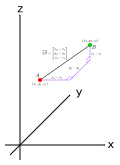
\includegraphics[width = 0.5\textwidth]{displacement_vector}
}
\end{tabular}

\textbf{Examples:}
\begin{itemize}
\item The displacement of point \(C(7, -1, 4)\) relative to point \(D(1, 0, -11)\) is:
\[\overrightarrow{DC} = \begin{bmatrix} 7 - 1 \\ (-1) - 0 \\ 4 - (-11) \end{bmatrix} = \begin{bmatrix} 6 \\ -1 \\ 15 \end{bmatrix}\]
\item The displacement from point \(X(6, -8, 7)\) to point \(Y(0, -10, 11)\) is:
\[\overrightarrow{XY} = \begin{bmatrix} 0 - 6 \\ (-10) - (-8) \\ 11 - 7 \end{bmatrix} = \begin{bmatrix} -6 \\ -2 \\ 4 \end{bmatrix}\]
\item The displacement from point \(B(9, 0, -1)\) to point \(C(12, -3, 5)\) is:
\[\overrightarrow{BC} = \begin{bmatrix} 12 - 9 \\ (-3) - 0 \\ 5 - (-1) \end{bmatrix} = \begin{bmatrix} 3 \\ -3 \\ 6 \end{bmatrix}\]
\item Given the vector \(\mathbf{u} = \begin{bmatrix} -8 \\ 5 \\ 1 \end{bmatrix}\), if the tail of the vector arrow is located at \((-2, -1, -5)\), then the head of the vector arrow is located at 
\[((-2)+(-8), (-1)+5, (-5)+1) = (-10, 4, -4)\]  
\end{itemize}

When the zero vector \(\mathbf{0}\) is envisioned as an arrow, the tail and end are the same point. The arrow has a length of \(0\), and has {\bf no direction}. 


\subsection*{Vector arithmetic}

When vectors are envisioned as arrows, the sum of two vectors is performed using the head-to-tail rule. Given two arbitrary vectors \(\mathbf{u}\) and \(\mathbf{v}\), the sum \(\mathbf{u} + \mathbf{v}\) is computed by moving the arrow that represents \(\mathbf{v}\) so that its tail is the same point as the head of the arrow that represents \(\mathbf{u}\). The arrow that represents \(\mathbf{u} + \mathbf{v}\) has the tail of \(\mathbf{u}\), and the had of \(\mathbf{v}\) as seen in the image below. In the image below, there is a triangle with vertices \(A(x_1, y_1, z_1)\), \(B(x_2, y_2, z_2)\), and \(C(x_3, y_3, z_3)\). The vector \(\mathbf{u}\) is the displacement from point \(A\) to \(B\), the vector \(\mathbf{v}\) is the displacement from \(B\) to \(C\), and the vector sum \(\mathbf{u} + \mathbf{v}\) is the displacement from \(A\) to \(C\). These displacements are:

\[\mathbf{u} = \overrightarrow{AB} = \begin{bmatrix} x_2 - x_1 \\ y_2 - y_1 \\ z_2 - z_1 \end{bmatrix} \quad\text{and}\quad \mathbf{v} = \overrightarrow{BC} = \begin{bmatrix} x_3 - x_2 \\ y_3 - y_2 \\ z_3 - z_2 \end{bmatrix} \quad\text{and}\quad \mathbf{u}+\mathbf{v} = \overrightarrow{AC} = \begin{bmatrix} x_3 - x_1 \\ y_3 - y_1 \\ z_3 - z_1 \end{bmatrix}\]

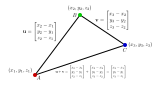
\includegraphics[width = \textwidth]{displacement_addition}


When vectors are envisioned as arrows, the multiplication of a scalar \(c\) with a vector \(\mathbf{u}\) is performed by increasing the length of \(\mathbf{u}\) by a factor of \(|c|\). If \(c\) is negative, then the direction is reversed. In the image below, there are \(3\) points in a straight line \(A\), \(B\), and \(C\). The vector \(\mathbf{u}\) is the displacement from point \(A\) to \(B\). The vector \(c\mathbf{u}\) is the displacement from point \(A\) to \(C\). The distance from \(A\) to \(C\) is \(c\) times the distance from \(A\) to \(B\), and the changes in the coordinates between the tail and head of the vector \(\overrightarrow{AB}\) are increased by a factor of \(c\) as well.

\[\mathbf{u} = \overrightarrow{AB} = \begin{bmatrix} \Delta x \\ \Delta y \\ \Delta z \end{bmatrix} \quad\text{and}\quad c\mathbf{u} = \overrightarrow{AC} = \begin{bmatrix} c\Delta x \\ c\Delta y \\ c\Delta z \end{bmatrix}\]

\begin{center}
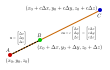
\includegraphics[width = 0.75\textwidth]{displacement_scalar_multiplication}
\end{center}


When vectors are envisioned as arrows, computing the negative of a vector simply involves reversing the orientation of the arrow. In the image below, there are two points \(A(x_1, y_1, z_1)\) and \(B(x_2, y_2, z_2)\). Vector \(\mathbf{u}\) is the displacement from point \(A\) to \(B\), and the vector \(-\mathbf{u}\) is the displacement from point \(B\) to \(A\).

\[\mathbf{u} = \overrightarrow{AB} = \begin{bmatrix} x_2 - x_1 \\ y_2 - y_1 \\ z_2 - z_1 \end{bmatrix} \quad\text{and}\quad -\mathbf{u} = \overrightarrow{BA} = \begin{bmatrix} x_1 - x_2 \\ y_1 - y_2 \\ z_1 - z_2 \end{bmatrix}\]

\begin{center}
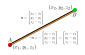
\includegraphics[width = 0.75\textwidth]{displacement_vector_negative}
\end{center}

Recall that the distributive laws hold for scalar multiplication. In the image below, the image on the left illustrates how for scalars \(c\) and \(k\), and vector \(\mathbf{v}\), that \((c + k)\mathbf{v} = c\mathbf{v} + k\mathbf{v}\). The image on the right illustrates how for scalar \(c\) and vectors \(\mathbf{u}\) and \(\mathbf{v}\), that \(c(\mathbf{u} + \mathbf{v}) = c\mathbf{u} + c\mathbf{v}\).

\begin{center}
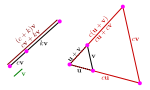
\includegraphics[width = 0.75\textwidth]{distributive_laws}   
\end{center}


Recall that a {\bf linear combination} of a set of vectors \(\{\mathbf{u}_1, \mathbf{u}_2, ..., \mathbf{u}_k\}\) is a weighted sum of the vectors from that set:
\[\alpha_1 \mathbf{u}_1 + \alpha_2 \mathbf{u}_2 + ... + \alpha_k \mathbf{u}_k\]

\begin{center}
\begin{tabular}{cc}
\parbox{0.5\textwidth}{
The image to the right depicts a rectangular prism. The goal is to use linear combinations of the vectors \(\mathbf{u}\), \(\mathbf{v}\), and \(\mathbf{w}\) to express the vectors \(\mathbf{p}\), \(\mathbf{q}\), \(\mathbf{r}\), and \(\mathbf{s}\). 
\begin{itemize}
\item[*] \(\mathbf{p} = \mathbf{v} - \mathbf{u} = (-1)\mathbf{u} + (1)\mathbf{v} + (0)\mathbf{w}\)
\item[*] \(\mathbf{q} = \mathbf{w} - \mathbf{v} = (0)\mathbf{u} + (-1)\mathbf{v} + (1)\mathbf{w}\)
\item[*] \(\mathbf{r} = \mathbf{u} + \mathbf{q} = (1)\mathbf{u} + (-1)\mathbf{v} + (1)\mathbf{w}\)
\item[*] \(\mathbf{s} = \mathbf{p} + \mathbf{q} = (-1)\mathbf{u} + (0)\mathbf{v} + (1)\mathbf{w}\)
\end{itemize}
} & \parbox{0.5\textwidth}{
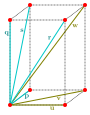
\includegraphics[width = 0.5\textwidth]{displacement_vector_lin_comb_example}
}
\end{tabular}
\end{center}



\subsection*{Parallelism}

When vectors are envisioned as arrows, two vectors \(\mathbf{u}\) and \(\mathbf{v}\) are considered to be ``parallel" if one vector is equal to the other vector multiplied by a nonzero scalar. There must exist a nonzero scalar \(c\) such that \(\mathbf{v} = c\mathbf{u}\). Consider the two nonzero vectors \(\mathbf{u} = \begin{bmatrix} u_x \\ u_y \\ u_z \end{bmatrix}\) and \(\mathbf{v} = \begin{bmatrix} v_x \\ v_y \\ v_z \end{bmatrix}\). To determine if \(\mathbf{u}\) and \(\mathbf{v}\) are parallel, the ratios between the corresponding components, \(v_x/u_x\), \(v_y/u_y\), and \(v_z/u_z\) need to be computed. Each of these ratios gives a value of \(c\). If all of these ratios are equal, then the vectors are parallel, with \(c\) being the common value. {\bf Any \(0/0\) ratio is a ``wildcard" and should be ignored.} 

\textbf{Examples:}
\begin{itemize}
%%%%%%%%%%%%%%%%%%%%
\item Given vectors \(\mathbf{u} = \begin{bmatrix} 6 \\ -2 \\ 8 \end{bmatrix}\) and \(\mathbf{v} = \begin{bmatrix} -9 \\ 3 \\ -12 \end{bmatrix}\), the ratios between the corresponding components are: 
\[v_x/u_x = -9/6 = -3/2 \quad\text{and}\quad v_y/u_y = 3/(-2) = -3/2 \quad\text{and}\quad v_z/u_z = -12/8 = -3/2\]
Since these ratios are all equal, \(\mathbf{u}\) and \(\mathbf{v}\) are {\bf parallel}.
%%%%%%%%%%%%%%%%%%%%
\item Given vectors \(\mathbf{u} = \begin{bmatrix} -3 \\ 15 \\ 6 \end{bmatrix}\) and \(\mathbf{v} = \begin{bmatrix} 7 \\ 35 \\ -14 \end{bmatrix}\), the ratios between the corresponding components are:
\[v_x/u_x = 7/(-3) = -7/3 \quad\text{and}\quad v_y/u_y = 35/15 = 7/3 \quad\text{and}\quad v_z/u_z = -14/6 = -7/3\]    
Since these ratios are not all equal, \(\mathbf{u}\) and \(\mathbf{v}\) are {\bf not parallel}.
%%%%%%%%%%%%%%%%%%%%
\item Given vectors \(\mathbf{u} = \begin{bmatrix} -18 \\ 0 \\ -27 \end{bmatrix}\) and \(\mathbf{v} = \begin{bmatrix} 10 \\ 0 \\ 15 \end{bmatrix}\), the ratios between the corresponding components are:
\[v_x/u_x = 10/(-18) = -5/9 \quad\text{and}\quad v_y/u_y = 0/0 \quad\text{and}\quad v_z/u_z = 15/(-27) = -5/9\]
The \(0/0\) reflects the fact that \(v_y = c u_y\) for any value of \(c\), and so the \(0/0\) ratio is a ``wildcard" that is ``equal" to any other ratio. The other ratios are equal so \(\mathbf{u}\) and \(\mathbf{v}\) are {\bf parallel}.
%%%%%%%%%%%%%%%%%%%%
\item Given vectors \(\mathbf{u} = \begin{bmatrix} -3 \\ 0 \\ 6 \end{bmatrix}\) and \(\mathbf{v} = \begin{bmatrix} 5 \\ 4 \\ -10 \end{bmatrix}\), the ratios between the corresponding components are:
\[v_x/u_x = 5/(-3) = -5/3 \quad\text{and}\quad v_y/u_y = 4/0 = \pm\infty \quad\text{and}\quad v_z/u_z = -10/6 = -5/3\]
Since these ratios are not all equal, \(\mathbf{u}\) and \(\mathbf{v}\) are {\bf not parallel}. In general, if one vector has a component that is \(0\), and the corresponding component is nonzero in the other vector, then it is immediately known that the vectors are not parallel.
\end{itemize}

{\bf Note that while the definition of parallelism given here requires that both vectors be nonzero, other contexts may allow for zero vectors to be parallel to nonzero vectors.}


\subsection*{Elementary basis vectors}

The ``elementary basis vectors" is a simple set of \(3\) vectors such that every vector that is a displacement in \(3\) dimensions is a linear combination of the elementary basis vectors. More specifically, the elementary basis vectors are:

\[\hat{\mathbf{i}} = \begin{bmatrix} 1 \\ 0 \\ 0 \end{bmatrix} \quad\text{and}\quad \hat{\mathbf{j}} = \begin{bmatrix} 0 \\ 1 \\ 0 \end{bmatrix} \quad\text{and}\quad \hat{\mathbf{k}} = \begin{bmatrix} 0 \\ 0\\ 1 \end{bmatrix}\]

Every vector \(\mathbf{u} = \begin{bmatrix} u_x \\ u_y \\ u_z \end{bmatrix}\) can be expressed as a linear combination of the elementary basis vectors \(\hat{\mathbf{i}}\), \(\hat{\mathbf{j}}\), and \(\hat{\mathbf{k}}\):
\[\mathbf{u} = \begin{bmatrix} u_x \\ u_y \\ u_z \end{bmatrix} = \begin{bmatrix} u_x \\ 0 \\ 0 \end{bmatrix} + \begin{bmatrix} 0 \\ u_y \\ 0 \end{bmatrix} + \begin{bmatrix} 0 \\ 0 \\ u_z \end{bmatrix} = u_x\begin{bmatrix} 1 \\ 0 \\ 0 \end{bmatrix} + u_y\begin{bmatrix} 0 \\ 1 \\ 0 \end{bmatrix} + u_z\begin{bmatrix} 0 \\ 0 \\ 1 \end{bmatrix} = u_x \hat{\mathbf{i}} + u_y \hat{\mathbf{j}} + u_z \hat{\mathbf{k}}\]



\subsection*{Vector magnitude}

When vectors are envisioned as arrows, the magnitude of the vector is the length of the arrow, which is equivalent to the Euclidean norm via the Pythagorean theorem, as demonstrated in the image below. 

If \(\mathbf{u} = \begin{bmatrix} u_x \\ u_y \\ u_z \end{bmatrix}\), then 
\[\|\mathbf{u}\| = \left\|\begin{bmatrix} u_x \\ u_y \\ u_z \end{bmatrix}\right\| = \sqrt{u_x^2 + u_y^2 + u_z^2}\]

Also, when given two points \(A(x_1, y_1, z_1)\) and \(B(x_2, y_2, z_2)\), the distance between points \(A\) and \(B\) is the magnitude of the displacement from \(A\) to \(B\): 
\[AB = \left\|\overrightarrow{AB}\right\| = \left\|\begin{bmatrix} x_2 - x_1 \\ y_2 - y_1 \\ z_2 - z_1 \end{bmatrix}\right\| = \sqrt{(x_2 - x_1)^2 + (y_2 - y_1)^2 + (z_2 - z_1)^2}\]

\begin{center}
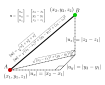
\includegraphics[width = 0.75\textwidth]{displacement_vector_magnitude}
\end{center}

\textbf{Examples:}
\begin{itemize}
\item Given the points \(A(3, 1, -4)\) and \(B(2, 4, -7)\), the displacement from \(A\) to \(B\) is \(\overrightarrow{AB} = \begin{bmatrix} 2 - 3 \\ 4 - 1 \\ (-7) - (-4) \end{bmatrix} = \begin{bmatrix} -1 \\ 3 \\ -3 \end{bmatrix}\). The distance between points \(A\) and \(B\) is the magnitude of \(\overrightarrow{AB}\) which is:
\[AB = \left\|\overrightarrow{AB}\right\| = \sqrt{(-1)^2 + 3^3 + (-3)^2} = \sqrt{1 + 9 + 9} = \sqrt{19}\]
\end{itemize}

A {\bf unit vector} is a vector with a magnitude of \(1\), and therefore the arrow associated with a unit vector has a length of \(1\). The normalization of a vector \(\mathbf{u}\) is defined as a vector that is \(\mathbf{u}\) multiplied by a positive scalar and has a magnitude of \(1\). This positive scalar is \(\frac{1}{\|\mathbf{u}\|}\), and the normalization of \(\mathbf{u}\) is \(\frac{\mathbf{u}}{\|\mathbf{u}\|}\). The normalization is an arrow that is parallel to \(\mathbf{u}\), but has a length of \(1\). Unit length vectors differ in direction alone, and the normalization of a vector is often used to quantify the vector's direction with the magnitude being ignored.  

\vspace{5mm}

If a vector with a magnitude of \(L\) and the direction of \(\mathbf{u}\) is what is desired, then \(L\frac{\mathbf{u}}{\|\mathbf{u}\|}\) has a magnitude of \(L\) and the direction of \(\mathbf{u}\). 

\begin{center}

\includegraphics[width = 0.75\textwidth]{displacement_vector_normalization}
\end{center}

\textbf{Examples:}
\begin{itemize}
%%%%%%%%%%%%%%%%%%%%%%%%%%%%%%%%
\item The normalization of the vector \(\mathbf{u} = \begin{bmatrix} -4 \\ 3 \end{bmatrix}\) is done as follows: First compute the magnitude:
\[\|\mathbf{u}\| = \left\|\begin{bmatrix} -4 \\ 3 \end{bmatrix}\right\| = \sqrt{(-4)^2 + 3^2} = \sqrt{16 + 9} = \sqrt{25} = 5\]  
Now normalize \(\mathbf{u}\):
\[\frac{\mathbf{u}}{\|\mathbf{u}\|} 
= \frac{1}{\|\mathbf{u}\|}\mathbf{u}   
= \frac{1}{5}\begin{bmatrix} -4 \\ 3 \end{bmatrix}
= \begin{bmatrix} -4/5 \\ 3/5 \end{bmatrix}\]
%%%%%%%%%%%%%%%%%%%%%%%%%%%%%%%%
\item The normalization of the vector \(\mathbf{u} = \begin{bmatrix} 3 \\ -1 \\ 2 \end{bmatrix}\) is done as follows: First compute the magnitude:
\[\|\mathbf{u}\| = \left\|\begin{bmatrix} 3 \\ -1 \\ 2 \end{bmatrix}\right\| = \sqrt{3^2 + (-1)^2 + 2^2} = \sqrt{9 + 1 + 4} = \sqrt{14}\]  
Now normalize \(\mathbf{u}\):
\[\frac{\mathbf{u}}{\|\mathbf{u}\|} 
= \frac{1}{\|\mathbf{u}\|}\mathbf{u}   
= \frac{1}{\sqrt{14}}\begin{bmatrix} 3 \\ -1 \\ 2 \end{bmatrix}
= \begin{bmatrix} 3/\sqrt{14} \\ -1/\sqrt{14} \\ 2/\sqrt{14} \end{bmatrix}\]
%%%%%%%%%%%%%%%%%%%%%%%%%%%%%%%%
\item The normalization of the vector \(\mathbf{v} = \begin{bmatrix} 2 \\ 1 \\ -2 \end{bmatrix}\) is done as follows: First compute the magnitude:
\[\|\mathbf{v}\| = \left\|\begin{bmatrix} 2 \\ 1 \\ -2 \end{bmatrix}\right\| = \sqrt{2^2 + 1^2 + (-2)^2} = \sqrt{4 + 1 + 4} = \sqrt{9} = 3\]  
Now normalize \(\mathbf{v}\):
\[\frac{\mathbf{v}}{\|\mathbf{v}\|} 
= \frac{1}{\|\mathbf{v}\|}\mathbf{v}   
= \frac{1}{3}\begin{bmatrix} 2 \\ 1 \\ -2 \end{bmatrix}
= \begin{bmatrix} 2/3 \\ 1/3 \\ -2/3 \end{bmatrix}\]
\end{itemize}




\subsection*{Deriving the components from the length and direction}

As previously discussed, there are two ways of quantifying vectors: 
\begin{itemize}
\item The first approach is to quantify a vector using its magnitude and direction. 
\item The second approach is to quantify a vector by listing its components. 
\end{itemize}
In many circumstances it is necessary to convert between the two forms.


Below, the process of deriving the components of a 2D vector when given its length and direction, is shown. There are 8 possible cases. It is important to know how to derive these cases instead of memorizing them. When a vector has:
\begin{itemize}
\item A length of \(r_1\), and an angle of \(\theta_1\) above the positive x-axis: \(\mathbf{v}_1 = \langle r_1\cos\theta_1, r_1\sin\theta_1 \rangle\)
\item A length of \(r_1\), and an angle of \(\phi_1\) right of the positive y-axis: \(\mathbf{v}_1 = \langle r_1\sin\phi_1, r_1\cos\phi_1 \rangle\)
\item A length of \(r_2\), and an angle of \(\theta_2\) left of the positive y-axis: \(\mathbf{v}_2 = \langle -r_2\sin\theta_2, r_2\cos\theta_2 \rangle\)
\item A length of \(r_2\), and an angle of \(\phi_2\) above the negative x-axis: \(\mathbf{v}_2 = \langle -r_2\cos\phi_2, r_2\sin\phi_2 \rangle\)
\item A length of \(r_3\), and an angle of \(\theta_3\) below the negative x-axis: \(\mathbf{v}_3 = \langle -r_3\cos\theta_3, -r_3\sin\theta_3 \rangle\)
\item A length of \(r_3\), and an angle of \(\phi_3\) left of the negative y-axis: \(\mathbf{v}_3 = \langle -r_3\sin\phi_3, -r_3\cos\phi_3 \rangle\)
\item A length of \(r_4\), and an angle of \(\theta_4\) right of the negative y-axis: \(\mathbf{v}_4 = \langle r_4\sin\theta_4, -r_4\cos\theta_4 \rangle\)
\item A length of \(r_4\), and an angle of \(\phi_4\) below the positive x-axis: \(\mathbf{v}_4 = \langle r_4\cos\phi_4, -r_4\sin\phi_4 \rangle\)
\end{itemize}
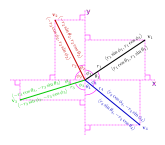
\includegraphics[width = \textwidth]{polar_vector_to_cartesian_vector}

\textbf{Examples:}
\begin{itemize}
%%%%%%%%%%%%%
\item Given a vector \(\mathbf{v}\) where \(\|\mathbf{v}\| = 5\) and the direction is \(\theta = 30^\circ\) above the positive x-axis, then \(\mathbf{v} = \langle 5\cos 30^\circ, 5\sin 30^\circ \rangle \approx \langle 4.33013, 2.50000 \rangle\)
%%%%%%%%%%%%%
\item Given a vector \(\mathbf{v}\) where \(\|\mathbf{v}\| = 6\) and the direction is \(\theta = 20^\circ\) left of the negative y-axis, then \(\mathbf{v} = \langle -6\sin 20^\circ, -6\cos 20^\circ \rangle \approx \langle -2.05212, -5.63816 \rangle\)
%%%%%%%%%%%%%
\item Given a vector \(\mathbf{v}\) where \(\|\mathbf{v}\| = 7\) and the direction is \(\theta = 25^\circ\) beneath the positive x-axis, then \(\mathbf{v} = \langle 7\cos 25^\circ, -7\sin 25^\circ \rangle \approx \langle 6.34415, -2.95833 \rangle\)
%%%%%%%%%%%%%
\item Given a vector \(\mathbf{v}\) where \(\|\mathbf{v}\| = 8\) and the direction is \(\theta = 53^\circ\) left of the positive y-axis, then \(\mathbf{v} = \langle -8\sin 53^\circ, 8\cos 53^\circ \rangle \approx \langle -6.38908, 4.81452 \rangle\)
\end{itemize}



\subsection*{Deriving the length and direction from the components}

Below, the process of deriving the length and direction of a 2D vector when given its components, is shown. Given a vector \(\mathbf{v} = \langle x, y \rangle\), the length of \(\mathbf{v}\) is always \(\|\mathbf{v}\| = \sqrt{x^2 + y^2}\). It is important to know how to derive these cases instead of memorizing them.
\begin{itemize}
\item When \(x \geq 0\) and \(y \geq 0\), the angle above the positive x-axis is \(\tan^{-1}(|y|/|x|)\), and the angle to the right of the positive y-axis is \(\tan^{-1}(|x|/|y|)\).
\item When \(x \leq 0\) and \(y \geq 0\), the angle to the left of the positive y-axis is \(\tan^{-1}(|x|/|y|)\), and the angle above the negative x-axis is \(\tan^{-1}(|y|/|x|)\).
\item When \(x \leq 0\) and \(y \leq 0\), the angle below the negative x-axis is \(\tan^{-1}(|y|/|x|)\), and the angle to the left of the negative y-axis is \(\tan^{-1}(|x|/|y|)\).
\item When \(x \geq 0\) and \(y \leq 0\), the angle to the right of the negative y-axis is \(\tan^{-1}(|x|/|y|)\), and the angle below the positive x-axis is \(\tan^{-1}(|y|/|x|)\).
\end{itemize}
In general, the angle measured against the \(x\)-axis, positive or negative, above or below, is \(\tan^{-1}(|y|/|x|)\), and the angle measured against the \(y\)-axis, positive or negative, right or left, is \(\tan^{-1}(|x|/|y|)\).

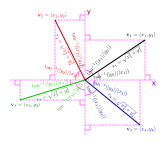
\includegraphics[width = \textwidth]{cartesian_vector_to_polar_vector}

\textbf{Examples:}
\begin{itemize}
%%%%%%%%%%%%%
\item Given the vector \(\mathbf{v} = \langle -2, 8 \rangle\), then the length is \(\|\mathbf{v}\| = \sqrt{(-2)^2 + 8^2} = \sqrt{4 + 64} = \sqrt{68} \approx 8.24621\), and the direction can be quantified as either \(\theta = \tan^{-1}(2/8) \approx 14.0362^\circ\) left of the positive y-axis, or \(\theta = \tan^{-1}(8/2) \approx 75.9638^\circ\) above the negative x-axis.
%%%%%%%%%%%%%
\item Given the vector \(\mathbf{v} = \langle -3, -5 \rangle\), then the length is \(\|\mathbf{v}\| = \sqrt{(-3)^2 + (-5)^2} = \sqrt{9 + 25} = \sqrt{34} \approx 5.83095\), and the direction can be quantified as either \(\theta = \tan^{-1}(5/3) \approx 59.0362^\circ\) below the negative x-axis, or \(\theta = \tan^{-1}(3/5) \approx 30.9638^\circ\) left of the negative y-axis.
%%%%%%%%%%%%%
\item Given the vector \(\mathbf{v} = \langle 6, 1 \rangle\), then the length is \(\|\mathbf{v}\| = \sqrt{6^2 + 1^2} = \sqrt{36 + 1} = \sqrt{37} \approx 6.08276\), and the direction can be quantified as either \(\theta = \tan^{-1}(1/6) \approx 9.46232^\circ\) above the positive x-axis, or \(\theta = \tan^{-1}(6/1) \approx 80.5377^\circ\) right of the positive y-axis.
%%%%%%%%%%%%%
\item Given the vector \(\mathbf{v} = \langle 3, -7 \rangle\), then the length is \(\|\mathbf{v}\| = \sqrt{3^2 + (-7)^2} = \sqrt{9 + 49} = \sqrt{58} \approx 7.61577\), and the direction can be quantified as either \(\theta = \tan^{-1}(3/7) \approx 23.1986^\circ\) right of the negative y-axis, or \(\theta = \tan^{-1}(7/3) \approx 66.8014^\circ\) below the positive x-axis.
%%%%%%%%%%%%%
\end{itemize}



\section*{Surfaces as vectors}

\begin{tabular}{cc}
\parbox{0.5\textwidth}{
A vector is a quantity with magnitude and direction. In most cases, a vector describes a displacement, which is the position of the head of an arrow relative to its tail. What often goes unnoticed is that another interpretation of magnitude and direction is to instead have the vector's magnitude denote area the area of a surface, and let the direction denote the direction in which the surface is facing. A flat surface with a preferred ``front" is quantified by a {\bf surface vector}, where the area is the magnitude, and the direction in which the surface is facing is the direction, as depicted on the right. More specifically the direction is perpendicular to the surface itself. The surface has a front and a back, and the direction of the surface vector is best described as an arrow sticking outwards from the ``front" of the surface. 
} & \parbox{0.5\textwidth}{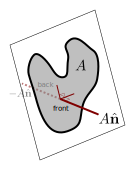
\includegraphics[width = 0.5\textwidth]{surface_vector_no_boundary}}
\end{tabular}

\begin{tabular}{cc}
\parbox{0.4\textwidth}{
To the right, is an image of an oriented surface that is not flat. The total surface vector is a linear combination (weighted sum) of the elementary basis vectors \(\hat{\mathbf{i}}\), \(\hat{\mathbf{j}}\), and \(\hat{\mathbf{k}}\). The sum of all the surface vectors that are parallel to the yz plane is: \(15\hat{\mathbf{i}} - 12\hat{\mathbf{i}} = 3\hat{\mathbf{i}}\). The sum of all the surface vectors that are parallel to the xz plane is: \(10\hat{\mathbf{j}}\). The sum of all the surface vectors that are parallel to the xy plane is: \(24\hat{\mathbf{k}}\). Therefore the total surface vector is:     
\[\mathbf{S} = 3\hat{\mathbf{i}} + 10\hat{\mathbf{j}} + 24\hat{\mathbf{k}}\]
} & \parbox{0.6\textwidth}{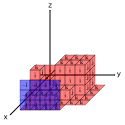
\includegraphics[width = 0.6\textwidth]{oriented_surface_1}}
\end{tabular}

From the above example, the 3 components of a surface vector can be derived by projecting the surface onto the yz-plane, xz-plane, and xy-plane respectively. This is similar to displacement vectors, where the 3 components of the displacement are the projections onto the x, y, and z axes respectively.   

\begin{tabular}{cc}
\parbox{0.5\textwidth}{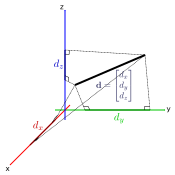
\includegraphics[width = 0.5\textwidth]{displacement_vector_components}} & 
\parbox{0.5\textwidth}{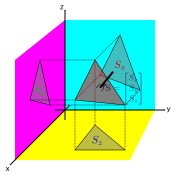
\includegraphics[width = 0.5\textwidth]{surface_vector_components}}
\end{tabular}



\section*{The dot product}

Now with regards to the dot product, given the two vectors \(\mathbf{u} = \begin{bmatrix} u_x \\ u_y \\ u_z \end{bmatrix}\) and \(\mathbf{v} = \begin{bmatrix} v_x \\ v_y \\ v_z \end{bmatrix}\), the dot product was defined to be \(\mathbf{u} \bullet \mathbf{v} = u_x v_x + u_y v_y + u_z v_z\). With regards to the understanding of vectors as arrows, if \(\theta\) is the angle between the arrows that represent \(\mathbf{u}\) and \(\mathbf{v}\), then 
\[\mathbf{u} \bullet \mathbf{v} = \|\mathbf{u}\|\|\mathbf{v}\|\cos\theta\]
{\bf These definitions are equivalent, and result in the same outcome.}

\begin{center}
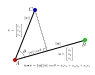
\includegraphics[width = 0.75\textwidth]{displacement_vector_dot_product}
\end{center}

One immediate observation is that \(\mathbf{u} \bullet \mathbf{u} = \|\mathbf{u}\|^2\). This observation can be easily derived from either definition.

The dot product is often used to compute the angle \(\theta\) between the two arrows represented by the two vectors \(\mathbf{u}\) and \(\mathbf{v}\). \(\mathbf{u} \bullet \mathbf{v} = u_x v_x + u_y v_y + u_z v_z\) is easy to compute, and:
\[\mathbf{u} \bullet \mathbf{v} = \|\mathbf{u}\|\|\mathbf{v}\|\cos\theta \iff \cos\theta = \frac{\mathbf{u} \bullet \mathbf{v}}{\|\mathbf{u}\| \|\mathbf{v}\|} \iff \theta = \cos^{-1}\left(\frac{\mathbf{u} \bullet \mathbf{v}}{\|\mathbf{u}\| \|\mathbf{v}\|}\right)\] 

Of particular interest is the scenario where \(\mathbf{u} \bullet \mathbf{v} = 0\) and \(\mathbf{u}\) and \(\mathbf{v}\) are both non-zero. In this case \(\theta = 90^\circ\), and the two vectors are said to be ``orthogonal", which is another way of saying perpendicular.

In addition, if \(\mathbf{u} \bullet \mathbf{v} > 0\), then \(\theta < 90^\circ\) so the angle between \(\mathbf{u}\) and \(\mathbf{v}\) is acute. If \(\mathbf{u} \bullet \mathbf{v} < 0\), then \(\theta > 90^\circ\) so the angle between \(\mathbf{u}\) and \(\mathbf{v}\) is obtuse.


\textbf{Examples:}
\begin{itemize}
%%%%%%%%%%%%%%%%%%%%%%%%%
\item If \(\mathbf{u} = \begin{bmatrix} -1 \\ 7 \\ 2 \end{bmatrix}\) and \(\mathbf{v} = \begin{bmatrix} 3 \\ 2 \\ 5 \end{bmatrix}\), then 
\[\mathbf{u} \bullet \mathbf{v} = (-1)(3) + (7)(2) + (2)(5) = -3 + 14 + 10 = 21\]
\[\|\mathbf{u}\| = \sqrt{(-1)^2 + 7^2 + 2^2} = \sqrt{1 + 49 + 4} = \sqrt{54}\]
\[\|\mathbf{v}\| = \sqrt{3^2 + 2^2 + 5^2} = \sqrt{9 + 4 + 25} = \sqrt{38}\]
\[\theta = \cos^{-1}\left(\frac{\mathbf{u} \bullet \mathbf{v}}{\|\mathbf{u}\| \|\mathbf{v}\|}\right) = \cos^{-1}\left(\frac{21}{(\sqrt{54})(\sqrt{38})}\right) \approx 62.3812^\circ\]
%%%%%%%%%%%%%%%%%%%%%%%%%
\item If \(\mathbf{u} = \begin{bmatrix} 5 \\ -2 \\ -1 \end{bmatrix}\) and \(\mathbf{v} = \begin{bmatrix} -3 \\ -10 \\ 5 \end{bmatrix}\), then 
\[\mathbf{u} \bullet \mathbf{v} = (5)(-3) + (-2)(-10) + (-1)(5) = -15 + 20 - 5 = 0\]
\(\mathbf{u}\) and \(\mathbf{v}\) are orthogonal, and hence \(\theta = 90^\circ\).
%%%%%%%%%%%%%%%%%%%%%%%%%
\item If \(\mathbf{u} = \begin{bmatrix} 5 \\ -3 \\ 1 \end{bmatrix}\) and \(\mathbf{v} = \begin{bmatrix} -1 \\ 2 \\ 5 \end{bmatrix}\), then 
\[\mathbf{u} \bullet \mathbf{v} = (5)(-1) + (-3)(2) + (1)(5) = -5 - 6 + 5 = -6\]
\[\|\mathbf{u}\| = \sqrt{5^2 + (-3)^2 + 1^2} = \sqrt{25 + 9 + 1} = \sqrt{35}\]
\[\|\mathbf{v}\| = \sqrt{(-1)^2 + 2^2 + 5^2} = \sqrt{1 + 4 + 25} = \sqrt{30}\]
\[\theta = \cos^{-1}\left(\frac{\mathbf{u} \bullet \mathbf{v}}{\|\mathbf{u}\| \|\mathbf{v}\|}\right) = \cos^{-1}\left(\frac{-6}{(\sqrt{35})(\sqrt{30})}\right) \approx 100.671^\circ\]
\end{itemize}

\vspace{5mm}

\textbf{Algebraic properties of the dot product include:}

\begin{centering}
\begin{itemize}
%%%%%%%%%%%%%%%%%%%%%%%%
\item Commutativity:
\[\mathbf{u} \bullet \mathbf{v} = \mathbf{v} \bullet \mathbf{u}\]
%%%%%%%%%%%%%%%%%%%%%%%%
\item Linearity in the first operand:
\begin{align*}
(\mathbf{u} + \mathbf{v}) \bullet \mathbf{w} = & \mathbf{u} \bullet \mathbf{w} + \mathbf{v} \bullet \mathbf{w} \\ 
(c\mathbf{u}) \bullet \mathbf{w} = & c(\mathbf{u} \bullet \mathbf{w}) 
\end{align*}
%%%%%%%%%%%%%%%%%%%%%%%%
\item Linearity in the second operand:
\begin{align*}
\mathbf{u} \bullet (\mathbf{v} + \mathbf{w}) = & \mathbf{u} \bullet \mathbf{v} + \mathbf{u} \bullet \mathbf{w} \\ 
\mathbf{u} \bullet (c\mathbf{v}) = & c(\mathbf{u} \bullet \mathbf{v}) 
\end{align*}
%%%%%%%%%%%%%%%%%%%%%%%%
\item A dot product with the zero vector always results in zero:
\begin{align*}
\mathbf{0} \bullet \mathbf{u} = & 0 \\ 
\mathbf{u} \bullet \mathbf{0} = & 0
\end{align*}
%%%%%%%%%%%%%%%%%%%%%%%%
\item The dot product of a vector with itself is always the square of its magnitude:
\[\mathbf{u} \bullet \mathbf{u} = \left\|\mathbf{u}\right\|^2\]
%%%%%%%%%%%%%%%%%%%%%%%%
\item Since \(\cos\theta\) can never escape the range \([-1, 1]\), it is the case that:
\[- \left\|\mathbf{u}\right\| \left\|\mathbf{v}\right\| \leq \mathbf{u} \bullet \mathbf{v} \leq \left\|\mathbf{u}\right\| \left\|\mathbf{v}\right\|\]
Moreover:
\begin{align*}
\theta = 0 \implies & \mathbf{u} \bullet \mathbf{v} = \|\mathbf{u}\| \|\mathbf{v}\| \\
\theta \in (0, \pi/2) \implies & \mathbf{u} \bullet \mathbf{v} \in (0, \|\mathbf{u}\| \|\mathbf{v}\|) \\ 
\theta = \pi/2 \implies & \mathbf{u} \bullet \mathbf{v} = 0 \quad\quad\quad\quad\quad\quad (\text{this is important}) \\
\theta \in (\pi/2, \pi) \implies & \mathbf{u} \bullet \mathbf{v} \in (- \|\mathbf{u}\| \|\mathbf{v}\|, 0) \\ 
\theta = \pi \implies & \mathbf{u} \bullet \mathbf{v} = - \|\mathbf{u}\| \|\mathbf{v}\|
\end{align*}
\end{itemize}
\end{centering}



One common application of the dot product is to compute the projection, or ``shadow", that one vector casts on another vector. In the image below, there is depicted two vectors \(\mathbf{u}\) and \(\mathbf{v}\). The assumption is that \(\mathbf{u}\) is a nonzero vector. The vector \(\mathbf{v}\) can be broken into 2 components, \(\text{proj}(\mathbf{v}|\mathbf{u})\) and \(\text{perp}(\mathbf{v}|\mathbf{u})\). The ``projection" \(\text{proj}(\mathbf{v}|\mathbf{u})\) is either \(\mathbf{0}\) or parallel to \(\mathbf{u}\). The ``perpendicular component" \(\text{perp}(\mathbf{v}|\mathbf{u})\) is either \(\mathbf{0}\) or is perpendicular to \(\mathbf{u}\).

\begin{center}
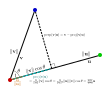
\includegraphics[width = 0.75\textwidth]{displacement_vector_proj_and_perp}
\end{center}

The projection \(\text{proj}(\mathbf{v}|\mathbf{u})\) is a multiple of \(\mathbf{u}\). The length of the projection is \(\|\mathbf{v}\|\cos\theta\) where \(\theta\) is the angle between \(\mathbf{u}\) and \(\mathbf{v}\). \(\|\mathbf{v}\|\cos\theta\) can be computed via:
\[\|\mathbf{v}\|\cos\theta = \frac{\|\mathbf{u}\|\|\mathbf{v}\|\cos\theta}{\|\mathbf{u}\|} = \frac{\mathbf{u} \bullet \mathbf{v}}{\|\mathbf{u}\|}\]
\(\frac{\mathbf{u}}{\|\mathbf{u}\|}\) is the normalization of \(\mathbf{u}\) that has the same direction as \(\mathbf{u}\) and a magnitude of \(1\). Multiplying \(\frac{\mathbf{u}}{\|\mathbf{u}\|}\) by the projection length gives the projection \(\text{proj}(\mathbf{v}|\mathbf{u})\):
\[\text{proj}(\mathbf{v}|\mathbf{u}) = (\|\mathbf{v}\|\cos\theta)\frac{\mathbf{u}}{\|\mathbf{u}\|} = \frac{\|\mathbf{u}\|\|\mathbf{v}\|\cos\theta}{\|\mathbf{u}\|^2}\mathbf{u} = \frac{\mathbf{u} \bullet \mathbf{v}}{\mathbf{u} \bullet \mathbf{u}}\mathbf{u}\]

One might ask the question: If \(\theta\) is obtuse, then the projection ``length" \(\|\mathbf{v}\|\cos\theta\) is negative. However in this case, the projection points in the opposite direction of \(\mathbf{u}\) so the negative sign does {\bf not} need to be removed.

The perpendicular component of \(\mathbf{v}\) remains when the projection is removed:
\[\text{perp}(\mathbf{v}|\mathbf{u}) = \mathbf{v} - \text{proj}(\mathbf{v}|\mathbf{u}) = \mathbf{v} - \frac{\mathbf{u} \bullet \mathbf{v}}{\mathbf{u} \bullet \mathbf{u}}\mathbf{u}\]

In summary, 
\[\text{proj}(\mathbf{v}|\mathbf{u}) = \frac{\mathbf{u} \bullet \mathbf{v}}{\mathbf{u} \bullet \mathbf{u}}\mathbf{u} \quad\text{and}\quad \text{perp}(\mathbf{v}|\mathbf{u}) = \mathbf{v} - \frac{\mathbf{u} \bullet \mathbf{v}}{\mathbf{u} \bullet \mathbf{u}}\mathbf{u}\]

If the magnitude of the projection is what is needed, then the magnitude is simply:
\[\|\text{proj}(\mathbf{v}|\mathbf{u})\| = \frac{|\mathbf{u} \bullet \mathbf{v}|}{\|\mathbf{u}\|}\]

If the magnitude of the perpendicular component is what is needed, then the magnitude can be computed from the magnitude of the projection via the Pythagorean theorem:
\[\|\text{perp}(\mathbf{v}|\mathbf{u})\| 
= \sqrt{\|\mathbf{v}\|^2 - \|\text{proj}(\mathbf{v}|\mathbf{u})\|^2} 
= \sqrt{\|\mathbf{v}\|^2 - \left(\frac{|\mathbf{u} \bullet \mathbf{v}|}{\|\mathbf{u}\|}\right)^2}
= \frac{\sqrt{\|\mathbf{u}\|^2\|\mathbf{v}\|^2 - (\mathbf{u} \bullet \mathbf{v})^2}}{\|\mathbf{u}\|}\]

\vspace{5mm}

If there is a line \(L\) that is parallel to \(\mathbf{u}\), and a point \(P\) whose displacement from another point on line \(L\) is \(\mathbf{v}\), then \(\|\text{perp}(\mathbf{v}|\mathbf{u})\|\) is the shortest distance from line \(L\) to point \(P\).

\vspace{5mm}

It is easy to prove that \(\mathbf{u}\) and \(\text{perp}(\mathbf{v}|\mathbf{u})\) are perpendicular using the dot product: 
\[\mathbf{u} \bullet \text{perp}(\mathbf{v}|\mathbf{u}) = 
\mathbf{u} \bullet \left(\mathbf{v} - \frac{\mathbf{u} \bullet \mathbf{v}}{\mathbf{u} \bullet \mathbf{u}}\mathbf{u}\right) = 
\mathbf{u} \bullet \mathbf{v} - \frac{\mathbf{u} \bullet \mathbf{v}}{\mathbf{u} \bullet \mathbf{u}}(\mathbf{u} \bullet \mathbf{u}) = 
0\]

\textbf{Examples:}
\begin{itemize}
%%%%%%%%%%%%%%%%%%%%%
\item Let \(\mathbf{u} = \begin{bmatrix} 2 \\ -2 \\ 1 \end{bmatrix}\) and \(\mathbf{v} = \begin{bmatrix} -7 \\ 3 \\ 4 \end{bmatrix}\). \\
\(\mathbf{u} \bullet \mathbf{u} = \|\mathbf{u}\|^2 = 2^2 + (-2)^2 + 1^2 = 4 + 4 + 1 = 9\), \\
\(\mathbf{v} \bullet \mathbf{v} = \|\mathbf{v}\|^2 = (-7)^2 + 3^2 + 4^2 = 49 + 9 + 16 = 74\), and \\
\(\mathbf{u} \bullet \mathbf{v} = (2)(-7) + (-2)(3) + (1)(4) = -14 - 6 + 4 = -16\). Therefore:
\[\text{proj}(\mathbf{v}|\mathbf{u}) = \frac{\mathbf{u} \bullet \mathbf{v}}{\mathbf{u} \bullet \mathbf{u}}\mathbf{u} = \frac{-16}{9}\begin{bmatrix} 2 \\ -2 \\ 1 \end{bmatrix} = \begin{bmatrix} -32/9 \\ 32/9 \\ -16/9 \end{bmatrix}\]
and 
\[\text{perp}(\mathbf{v}|\mathbf{u}) = \mathbf{v} - \text{proj}(\mathbf{v}|\mathbf{u}) = \begin{bmatrix} -7 \\ 3 \\ 4 \end{bmatrix} - \begin{bmatrix} -32/9 \\ 32/9 \\ -16/9 \end{bmatrix} = \begin{bmatrix} -31/9 \\ -5/9 \\ 52/9 \end{bmatrix}\]
The magnitude of the projection is:
\[\|\text{proj}(\mathbf{v}|\mathbf{u})\| = \frac{|\mathbf{u} \bullet \mathbf{v}|}{\|\mathbf{u}\|} = \frac{|-16|}{3} = \frac{16}{3}\]
The magnitude of the perpendicular component is:
\[\|\text{perp}(\mathbf{v}|\mathbf{u})\| = \frac{\sqrt{\|\mathbf{u}\|^2\|\mathbf{v}\|^2 - (\mathbf{u} \bullet \mathbf{v})^2}}{\|\mathbf{u}\|} = \frac{\sqrt{(9)(74) - (-16)^2}}{3} = \frac{\sqrt{410}}{3}\]
%%%%%%%%%%%%%%%%%%%%%
\item Let \(\mathbf{u} = \begin{bmatrix} -3 \\ -2 \\ 1 \end{bmatrix}\) and \(\mathbf{v} = \begin{bmatrix} -1 \\ 5 \\ -7 \end{bmatrix}\). \\
\(\mathbf{u} \bullet \mathbf{u} = \|\mathbf{u}\|^2 = (-3)^2 + (-2)^2 + 1^2 = 9 + 4 + 1 = 14\), \\
\(\mathbf{v} \bullet \mathbf{v} = \|\mathbf{v}\|^2 = (-1)^2 + 5^2 + (-7)^2 = 1 + 25 + 49 = 75\), and \\ 
\(\mathbf{u} \bullet \mathbf{v} = (-3)(-1) + (-2)(5) + (1)(-7) = 3 - 10 - 7 = -14\). Therefore:
\[\text{proj}(\mathbf{v}|\mathbf{u}) = \frac{\mathbf{u} \bullet \mathbf{v}}{\mathbf{u} \bullet \mathbf{u}}\mathbf{u} = \frac{-14}{14}\begin{bmatrix} -3 \\ -2 \\ 1 \end{bmatrix} = \begin{bmatrix} 3 \\ 2 \\ -1 \end{bmatrix}\]
and 
\[\text{perp}(\mathbf{v}|\mathbf{u}) = \mathbf{v} - \text{proj}(\mathbf{v}|\mathbf{u}) = \begin{bmatrix} -1 \\ 5 \\ -7 \end{bmatrix} - \begin{bmatrix} 3 \\ 2 \\ -1 \end{bmatrix} = \begin{bmatrix} -4 \\ 3 \\ -6 \end{bmatrix}\]
The magnitude of the projection is:
\[\|\text{proj}(\mathbf{v}|\mathbf{u})\| = \frac{|\mathbf{u} \bullet \mathbf{v}|}{\|\mathbf{u}\|} = \frac{|-14|}{\sqrt{14}} = \sqrt{14}\]
The magnitude of the perpendicular component is:
\[\|\text{perp}(\mathbf{v}|\mathbf{u})\| = \frac{\sqrt{\|\mathbf{u}\|^2\|\mathbf{v}\|^2 - (\mathbf{u} \bullet \mathbf{v})^2}}{\|\mathbf{u}\|} = \frac{\sqrt{(14)(75) - (-14)^2}}{\sqrt{14}} = \frac{\sqrt{854}}{\sqrt{14}} = \sqrt{61}\]
%%%%%%%%%%%%%%%%%%%%%
\item Let \(\mathbf{u} = \begin{bmatrix} 1 \\ -3 \\ 0 \end{bmatrix}\) and \(\mathbf{v} = \begin{bmatrix} 5 \\ 2 \\ -7 \end{bmatrix}\). \\
\(\mathbf{u} \bullet \mathbf{u} = \|\mathbf{u}\|^2 = 1^2 + (-3)^2 + 0^2 = 1 + 9 + 0 = 10\), \\
\(\mathbf{v} \bullet \mathbf{v} = \|\mathbf{v}\|^2 = 5^2 + 2^2 + (-7)^2 = 25 + 4 + 49 = 78\), and \\
\(\mathbf{u} \bullet \mathbf{v} = (1)(5) + (-3)(2) + (0)(-7) = 5 - 6 + 0 = -1\). Therefore: 
\[\text{proj}(\mathbf{v}|\mathbf{u}) = \frac{\mathbf{u} \bullet \mathbf{v}}{\mathbf{u} \bullet \mathbf{u}}\mathbf{u} = \frac{-1}{10}\begin{bmatrix} 1 \\ -3 \\ 0 \end{bmatrix} = \begin{bmatrix} -1/10 \\ 3/10 \\ 0 \end{bmatrix}\]  
and 
\[\text{perp}(\mathbf{v}|\mathbf{u}) = \mathbf{v} - \text{proj}(\mathbf{v}|\mathbf{u}) = \begin{bmatrix} 5 \\ 2 \\ -7 \end{bmatrix} - \begin{bmatrix} -1/10 \\ 3/10 \\ 0 \end{bmatrix} = \begin{bmatrix} 51/10 \\ 17/10 \\ -7 \end{bmatrix}\]
The magnitude of the projection is:
\[\|\text{proj}(\mathbf{v}|\mathbf{u})\| = \frac{|\mathbf{u} \bullet \mathbf{v}|}{\|\mathbf{u}\|} = \frac{|-1|}{\sqrt{10}} = \frac{1}{\sqrt{10}}\]
The magnitude of the perpendicular component is:
\[\|\text{perp}(\mathbf{v}|\mathbf{u})\| = \frac{\sqrt{\|\mathbf{u}\|^2\|\mathbf{v}\|^2 - (\mathbf{u} \bullet \mathbf{v})^2}}{\|\mathbf{u}\|} = \frac{\sqrt{(10)(78) - (-1)^2}}{\sqrt{10}} = \frac{\sqrt{779}}{\sqrt{10}} = \sqrt{\frac{779}{10}}\]
\end{itemize}


\begin{tabular}{cc}
\parbox{0.5\textwidth}{Given a prism with a cross-sectional area of \(A\) and a length of \(d\), the volume is \(V = A \cdot d\). This formula can be generalized to cross-sectional surfaces and displacement lengths. Consider a surface with a surface vector of \(\mathbf{A}\), and consider a displacement of \(\mathbf{d}\). ``Extrude" the surface vector \(\mathbf{A}\) along the displacement \(\mathbf{d}\), as depicted in the image to the right to create a volume. This volume is \(V = \mathbf{A} \bullet \mathbf{d}\). If the displacement \(\mathbf{d}\) is opposite to the direction faced by \(\mathbf{A}\), then the resultant volume is {\bf negative}. The actual volume is the absolute value \(V = \left|\mathbf{A} \bullet \mathbf{d}\right|\). The so called ``signed volume" \(\mathbf{A} \bullet \mathbf{d}\) is useful in other cases.
} & \parbox{0.5\textwidth}{
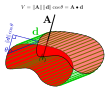
\includegraphics[width = 0.5\textwidth]{surface_displacement_product}
}
\end{tabular}


Lastly, the equivalence of the two definitions \(\mathbf{u} \bullet \mathbf{v} = u_x v_x + u_y v_y + u_z v_z\) and \(\mathbf{u} \bullet \mathbf{v} = \|\mathbf{u}\|\|\mathbf{v}\|\cos\theta\) will be demonstrated. While it will not be shown here, the definition \(\mathbf{u} \bullet \mathbf{v} = \|\mathbf{u}\|\|\mathbf{v}\|\cos\theta\) can be shown to give rise to the distributive law, \(\mathbf{u} \bullet (\mathbf{v} + \mathbf{w}) = \mathbf{u} \bullet \mathbf{v} + \mathbf{u} \bullet \mathbf{w}\), via the observation that the projection of \(\mathbf{v} + \mathbf{w}\) onto \(\mathbf{u}\) is the sum of the projections of \(\mathbf{v}\) and \(\mathbf{w}\) onto \(\mathbf{u}\): \(\text{proj}(\mathbf{v} + \mathbf{w} | \mathbf{u}) = \text{proj}(\mathbf{v} | \mathbf{u}) + \text{proj}(\mathbf{w} | \mathbf{u})\)

Both \(\mathbf{u}\) and \(\mathbf{v}\) can be expressed as linear combinations of the elementary basis vectors:
\[\mathbf{u} = u_x \hat{\mathbf{i}} + u_y \hat{\mathbf{j}} + u_z \hat{\mathbf{k}} \quad\text{and}\quad \mathbf{v} = v_x \hat{\mathbf{i}} + v_y \hat{\mathbf{j}} + v_z \hat{\mathbf{k}}\]

\begin{center}
\begin{tabular}{cc}
\parbox{0.5\textwidth}{
Using the distributive law, 
\begin{align*}
\mathbf{u} \bullet \mathbf{v} = & (u_x \hat{\mathbf{i}} + u_y \hat{\mathbf{j}} + u_z \hat{\mathbf{k}}) \bullet (v_x \hat{\mathbf{i}} + v_y \hat{\mathbf{j}} + v_z \hat{\mathbf{k}}) \\ 
= & \;\;\;\; u_x v_x (\hat{\mathbf{i}} \bullet \hat{\mathbf{i}}) + u_x v_y (\hat{\mathbf{i}} \bullet \hat{\mathbf{j}}) + u_x v_z (\hat{\mathbf{i}} \bullet \hat{\mathbf{k}}) \\
& + u_y v_x (\hat{\mathbf{j}} \bullet \hat{\mathbf{i}}) + u_y v_y (\hat{\mathbf{j}} \bullet \hat{\mathbf{j}}) + u_y v_z (\hat{\mathbf{j}} \bullet \hat{\mathbf{k}}) \\ 
& + u_z v_x (\hat{\mathbf{k}} \bullet \hat{\mathbf{i}}) + u_z v_y (\hat{\mathbf{k}} \bullet \hat{\mathbf{j}}) + u_z v_z (\hat{\mathbf{k}} \bullet \hat{\mathbf{k}}) \\ 
= & \;\;\;\; u_x v_x (1) + u_x v_y (0) + u_x v_z (0) \\
& + u_y v_x (0) + u_y v_y (1) + u_y v_z (0) \\ 
& + u_z v_x (0) + u_z v_y (0) + u_z v_z (1) \\ 
= & u_x v_x + u_y v_y + u_z v_z
\end{align*}} & \parbox{0.5\textwidth}{
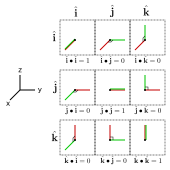
\includegraphics[width = 0.5\textwidth]{elementary_vector_dot_products}
}
\end{tabular}
Therefore:
\[\|\mathbf{u}\|\|\mathbf{v}\|\cos\theta = u_x v_x + u_y v_y + u_z v_z\]
\end{center}





\section*{The cross product}

%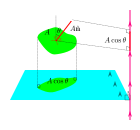
\includegraphics[width = 0.5\textwidth]{line_plane_duality}


%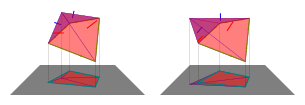
\includegraphics[width = \textwidth]{projecting_oriented_surfaces_onto_oriented_flat_planes_1}

Given a rectangle with dimensions \(u\) and \(v\), the area is \(A = u \times v\). Now let \(\mathbf{u}\) and \(\mathbf{v}\) denote displacement vectors. The parallelogram where one pair of sides each corresponds to the displacement \(\mathbf{u}\), and the other pair of sides corresponds to the displacement \(\mathbf{v}\), has a {\bf surface vector} that is the {\bf cross product} of \(\mathbf{u}\) and \(\mathbf{v}\):

\[\mathbf{A} = \mathbf{u} \times \mathbf{v}\]

Like with the dot product \(\theta\) will denote the angle between \(\mathbf{u}\) and \(\mathbf{v}\). The area of this parallelogram, as depicted in the image below is \(\|\mathbf{u}\| \|\mathbf{v}\| \sin\theta\), so the magnitude of the cross product is:

\[\left\|\mathbf{u} \times \mathbf{v}\right\| = \|\mathbf{u}\| \|\mathbf{v}\| \sin\theta\] 

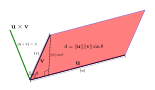
\includegraphics[scale = 1]{cross_product}

%\includegraphics[scale = 1]{cross_product_2}

The direction is perpendicular to the parallelogram, which also means that the direction is perpendicular to both \(\mathbf{u}\) and \(\mathbf{v}\). The surface has two sides/faces. Which side is the ``front", and is the direction of the cross product? The ``front" is determined by the {\bf right hand rule}. There are two descriptions of the right hand rule:

\begin{tabular}{cc}
\parbox{0.5\textwidth}{
Hold your right hand so that your thumb is (approximately) in the direction of \(\mathbf{u}\), and your fingers are (approximately) in the direction of \(\mathbf{v}\). Your palm is the parallelogram's front, and the back of your hand is the parallelogram's back.  
} & \parbox{0.4\textwidth}{
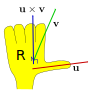
\includegraphics[width = 0.4\textwidth]{right_hand_rule_1}
}
\end{tabular}

\begin{tabular}{cc}
\parbox{0.3\textwidth}{
Grab with your right hand a bar that is perpendicular to \(\mathbf{u}\) and \(\mathbf{v}\) as shown on the right. Ensure that the angle between \(\mathbf{u}\) and \(\mathbf{v}\) is beneath your knuckles, that \(\mathbf{u}\) passes through the back of your hand, and that \(\mathbf{v}\) passes through your fingers. Your thumb will point in the direction of \(\mathbf{u} \times \mathbf{v}\). 
} & \parbox{0.6\textwidth}{
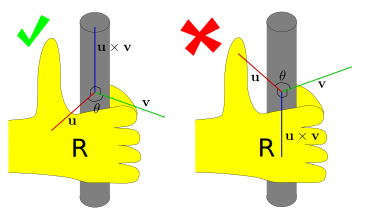
\includegraphics[width = 0.6\textwidth]{right_hand_rule_2}
}
\end{tabular}

\vspace{5mm}

It will be assumed that \(\hat{\mathbf{i}} \times \hat{\mathbf{j}} = \hat{\mathbf{k}}\). When this is true, the coordinate system is said to be {\bf right-handed}. If \(\hat{\mathbf{i}} \times \hat{\mathbf{j}} = -\hat{\mathbf{k}}\), then the coordinate system is {\bf left-handed}. All coordinate systems that we will use will be ``right-handed".  

\vspace{5mm}

Unlike the dot product, reversing the order of the factors in the cross product flips the sign of the product. This can be easily demonstrated via the right hand rule. 
\[\mathbf{u} \times \mathbf{v} = -(\mathbf{v} \times \mathbf{u})\]
The property is also referred to as ``anti-commutativity".

Moreover, since the cross product \(\mathbf{u} \times \mathbf{v}\) is perpendicular to both \(\mathbf{u}\) and \(\mathbf{v}\), the dot product of \(\mathbf{u}\) and \(\mathbf{v}\) with \(\mathbf{u} \times \mathbf{v}\) is \(0\):
\[\mathbf{u} \bullet (\mathbf{u} \times \mathbf{v}) = 0 \quad\quad\text{and}\quad\quad \mathbf{v} \bullet (\mathbf{u} \times \mathbf{v}) = 0\]

Other algebraic rules (not all of which will be proven) include:

\begin{centering}
\begin{itemize}
%%%%%%%%%%%%%%%%%%%%%%%%
%\item Anti-commutativity:
%\[\mathbf{u} \times \mathbf{v} = -(\mathbf{v} \times \mathbf{u})\]
%%%%%%%%%%%%%%%%%%%%%%%%
\item Linearity in the first operand:
\begin{align*}
(\mathbf{u} + \mathbf{v}) \times \mathbf{w} = & \mathbf{u} \times \mathbf{w} + \mathbf{v} \times \mathbf{w} \\ 
(c\mathbf{u}) \times \mathbf{w} = & c(\mathbf{u} \times \mathbf{w}) 
\end{align*}
%%%%%%%%%%%%%%%%%%%%%%%%
\item Linearity in the second operand:
\begin{align*}
\mathbf{u} \times (\mathbf{v} + \mathbf{w}) = & \mathbf{u} \times \mathbf{v} + \mathbf{u} \times \mathbf{w} \\ 
\mathbf{u} \times (c\mathbf{v}) = & c(\mathbf{u} \times \mathbf{v}) 
\end{align*}
%%%%%%%%%%%%%%%%%%%%%%%%
\item A cross product with the zero vector always results in the zero vector:
\begin{align*}
\mathbf{0} \times \mathbf{u} = & \mathbf{0} \\ 
\mathbf{u} \times \mathbf{0} = & \mathbf{0}
\end{align*}
%%%%%%%%%%%%%%%%%%%%%%%%
\item The cross product of a vector with itself is always the zero vector, since the parallelogram is simply a flat line and \(\theta = 0\):
\[\mathbf{u} \times \mathbf{u} = \mathbf{0}\]
moreover, if \(\mathbf{u}\) and \(\mathbf{v}\) are parallel, then \(\mathbf{u} \times \mathbf{v} = \mathbf{0}\)
%%%%%%%%%%%%%%%%%%%%%%%%
\item Since \(\sin\theta\) can never escape the range \([-1, 1]\), it is the case that:
\[0 \leq \left\|\mathbf{u} \times \mathbf{v}\right\| \leq \left\|\mathbf{u}\right\| \left\|\mathbf{v}\right\|\]
\end{itemize}
\end{centering}

The distributive law for the cross product can be used to derive a simple formula for the cross product:

Both \(\mathbf{u}\) and \(\mathbf{v}\) can be expressed as linear combinations of the elementary basis vectors:
\[\mathbf{u} = \begin{bmatrix} u_x \\ u_y \\ u_z \end{bmatrix} = u_x \hat{\mathbf{i}} + u_y \hat{\mathbf{j}} + u_z \hat{\mathbf{k}} \quad\text{and}\quad \mathbf{v} = \begin{bmatrix} v_x \\ v_y \\ v_z \end{bmatrix} = v_x \hat{\mathbf{i}} + v_y \hat{\mathbf{j}} + v_z \hat{\mathbf{k}}\]

\begin{center}
\begin{tabular}{cc}
\parbox{0.5\textwidth}{
Using the distributive law, 
\begin{align*}
\mathbf{u} \times \mathbf{v} = & (u_x \hat{\mathbf{i}} + u_y \hat{\mathbf{j}} + u_z \hat{\mathbf{k}}) \times (v_x \hat{\mathbf{i}} + v_y \hat{\mathbf{j}} + v_z \hat{\mathbf{k}}) \\ 
= & \;\;\;\; u_x v_x (\hat{\mathbf{i}} \times \hat{\mathbf{i}}) + u_x v_y (\hat{\mathbf{i}} \times \hat{\mathbf{j}}) + u_x v_z (\hat{\mathbf{i}} \times \hat{\mathbf{k}}) \\
& + u_y v_x (\hat{\mathbf{j}} \times \hat{\mathbf{i}}) + u_y v_y (\hat{\mathbf{j}} \times \hat{\mathbf{j}}) + u_y v_z (\hat{\mathbf{j}} \times \hat{\mathbf{k}}) \\ 
& + u_z v_x (\hat{\mathbf{k}} \times \hat{\mathbf{i}}) + u_z v_y (\hat{\mathbf{k}} \times \hat{\mathbf{j}}) + u_z v_z (\hat{\mathbf{k}} \times \hat{\mathbf{k}}) \\ 
= & \;\;\;\; u_x v_x (\mathbf{0}) + u_x v_y (\mathbf{k}) + u_x v_z (-\mathbf{j}) \\
& + u_y v_x (-\hat{\mathbf{k}}) + u_y v_y (\mathbf{0}) + u_y v_z (\hat{\mathbf{i}}) \\ 
& + u_z v_x (\hat{\mathbf{j}}) + u_z v_y (-\hat{\mathbf{i}}) + u_z v_z (\mathbf{0}) \\ 
= & (u_y v_z - u_z v_y)\hat{\mathbf{i}} + (u_z v_x - u_x v_z)\hat{\mathbf{j}} \\
& \quad + (u_x v_y - u_y v_x)\hat{\mathbf{k}}
\end{align*}} & \parbox{0.5\textwidth}{
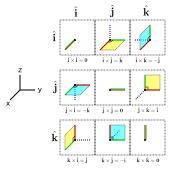
\includegraphics[width = 0.5\textwidth]{elementary_vector_cross_products}
}
\end{tabular}
Therefore:
\[\mathbf{u} \times \mathbf{v} = \begin{bmatrix} u_x \\ u_y \\ u_z \end{bmatrix} \times \begin{bmatrix} v_x \\ v_y \\ v_z \end{bmatrix} = (u_y v_z - u_z v_y)\hat{\mathbf{i}} + (u_z v_x - u_x v_z)\hat{\mathbf{j}} + (u_x v_y - u_y v_x)\hat{\mathbf{k}}
= \begin{bmatrix} u_y v_z - u_z v_y \\ u_z v_x - u_x v_z \\ u_x v_y - u_y v_x \end{bmatrix}\]
\end{center}

To help remember the cross product formula, the following mnemonics will be used:
\begin{center}
\begin{tabular}{cc}
\parbox{0.6\textwidth}{
As depicted on the right, order the elementary basis vectors \(\hat{\mathbf{i}}\), \(\hat{\mathbf{j}}\), and \(\hat{\mathbf{k}}\) in a cyclical manner where \(\hat{\mathbf{i}}\) is followed by \(\hat{\mathbf{j}}\), which is followed by \(\hat{\mathbf{k}}\), which is again followed by \(\hat{\mathbf{i}}\): 
\[\hat{\mathbf{i}} \rightarrow \hat{\mathbf{j}} \rightarrow \hat{\mathbf{k}} \rightarrow \hat{\mathbf{i}}\] 

The cross product of an elementary basis vector with itself is always \(\mathbf{0}\).  

The cross product of two different elementary basis vectors is a multiple of the remaining basis vector. If the multiplicands are in order, the coefficient is \(+1\):
\[\hat{\mathbf{i}} \times \hat{\mathbf{j}} = \hat{\mathbf{k}} \quad\text{and}\quad \hat{\mathbf{j}} \times \hat{\mathbf{k}} = \hat{\mathbf{i}} \quad\text{and}\quad \hat{\mathbf{k}} \times \hat{\mathbf{i}} = \hat{\mathbf{j}}\] 
If the multiplicands are out of order, the coefficient is \(-1\):
\[\hat{\mathbf{j}} \times \hat{\mathbf{i}} = -\hat{\mathbf{k}} \quad\text{and}\quad \hat{\mathbf{k}} \times \hat{\mathbf{j}} = -\hat{\mathbf{i}} \quad\text{and}\quad \hat{\mathbf{i}} \times \hat{\mathbf{k}} = -\hat{\mathbf{j}}\] 
It is important to note that the correct ordering of \(\hat{\mathbf{i}}\) and \(\hat{\mathbf{k}}\) is \(\hat{\mathbf{k}}\) followed by \(\hat{\mathbf{i}}\).
} & \parbox{0.4\textwidth}{
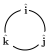
\includegraphics[width = 0.4\textwidth]{i_j_k_cycle}
}
\end{tabular}
\end{center}

\begin{center}
\begin{tabular}{cc}
\parbox{0.6\textwidth}{
To memorize
\[\begin{bmatrix} u_x \\ u_y \\ u_z \end{bmatrix} \times \begin{bmatrix} v_x \\ v_y \\ v_z \end{bmatrix} = \begin{bmatrix} u_y v_z - u_z v_y \\ u_z v_x - u_x v_z \\ u_x v_y - u_y v_x \end{bmatrix}\]
order the dimensions \(x\), \(y\), and \(z\) in a cyclical manner where \(x\) is followed by \(y\), which is followed by \(z\), which is again followed by \(x\). 
\[x \rightarrow y \rightarrow z \rightarrow x\] 

To compute a component of \(\mathbf{u} \times \mathbf{v}\), one must consider the components of \(\mathbf{u}\) and \(\mathbf{v}\) that \emph{do not} include the current component. The product of components that \emph{do not} correspond to each other are computed. The product of components where the dimensions are in order gets the coefficient of \(+1\):
\[+u_x v_y \quad\quad\quad +u_y v_z \quad\quad\quad +u_z v_x\]
 while the product of the components where the dimensions are out of order gets the coefficient of \(-1\):
\[-u_y v_x \quad\quad\quad -u_z v_y \quad\quad\quad -u_x v_z\]
It is important to note that the correct ordering of \(x\) and \(z\) is \(z\) followed by \(x\).
} & \parbox{0.4\textwidth}{
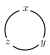
\includegraphics[width = 0.4\textwidth]{x_y_z_cycle}
}
\end{tabular}
\end{center}



\textbf{Examples:}
\begin{itemize}
%%%%%%%%%%%%%%%%%%%%%%
\item If \(\mathbf{u} = \begin{bmatrix} 3 \\ -1 \\ 2 \end{bmatrix}\) and \(\mathbf{v} = \begin{bmatrix} 4 \\ 2 \\ -1 \end{bmatrix}\), then
\[\mathbf{u} \times \mathbf{v} = \begin{bmatrix} (-1)(-1) - (2)(2) \\ (2)(4) - (3)(-1) \\ (3)(2) - (-1)(4) \end{bmatrix} = \begin{bmatrix} 1 - 4 \\ 8 + 3 \\ 6 + 4 \end{bmatrix} = \begin{bmatrix} -3 \\ 11 \\ 10 \end{bmatrix}\]
Since the cross product is perpendicular to both operands, the dot products of the cross product with the operands must be \(0\):
\[\mathbf{u} \bullet (\mathbf{u} \times \mathbf{v}) = -9 - 11 + 20 = 0 \quad\quad\text{and}\quad\quad \mathbf{v} \bullet (\mathbf{u} \times \mathbf{v}) = -12 + 22 - 10 = 0\]
This can be used to check our work.
%%%%%%%%%%%%%%%%%%%%%%
\item If \(\mathbf{u} = \begin{bmatrix} 4 \\ -1 \\ -3 \end{bmatrix}\) and \(\mathbf{v} = \begin{bmatrix} 5 \\ -2 \\ -1 \end{bmatrix}\), then
\[\mathbf{u} \times \mathbf{v} = \begin{bmatrix} (-1)(-1) - (-3)(-2) \\ (-3)(5) - (4)(-1) \\ (4)(-2) - (-1)(5) \end{bmatrix} = \begin{bmatrix} 1 - 6 \\ -15 + 4 \\ -8 + 5 \end{bmatrix} = \begin{bmatrix} -5 \\ -11 \\ -3 \end{bmatrix}\]
Since the cross product is perpendicular to both operands, the dot products of the cross product with the operands must be \(0\):
\[\mathbf{u} \bullet (\mathbf{u} \times \mathbf{v}) = -20 + 11 + 9 = 0 \quad\quad\text{and}\quad\quad \mathbf{v} \bullet (\mathbf{u} \times \mathbf{v}) = -25 + 22 + 3 = 0\]
This demonstrates that our computed cross product is likely free of errors.
\end{itemize}

\vspace{5mm}

With the cross product, given arbitrary points \(P\), \(Q\), and \(R\), the area of the triangle \(\Delta PQR\) can be computed. First compute the displacements \(\overrightarrow{PQ}\) and \(\overrightarrow{PR}\). The triangle \(\Delta PQR\) is half of the parallelogram bounded by \(\overrightarrow{PQ}\) and \(\overrightarrow{PR}\), so its area is \(\frac{1}{2}\left\|\overrightarrow{PQ} \times \overrightarrow{PR}\right\|\). 

\textbf{Examples:}
\begin{itemize}
\item Let the points \(P\), \(Q\), and \(R\) be:
\[P(3, 0, 0) \quad\text{and}\quad Q(0, 4, 0) \quad\text{and}\quad R(0, 0, 5)\]
\[\overrightarrow{PQ} = \begin{bmatrix} -3 \\ 4 \\ 0 \end{bmatrix} \quad\text{and}\quad \overrightarrow{PR} = \begin{bmatrix} -3 \\ 0 \\ 5 \end{bmatrix}\]
\[\overrightarrow{PQ} \times \overrightarrow{PR} = \begin{bmatrix} (4)(5) - (0)(0) \\ (0)(-3) - (-3)(5) \\ (-3)(0) - (4)(-3) \end{bmatrix} = \begin{bmatrix} 20 - 0 \\ 0 + 15 \\ 0 + 12 \end{bmatrix} = \begin{bmatrix} 20 \\ 15 \\ 12 \end{bmatrix}\]
\[\left\|\overrightarrow{PQ} \times \overrightarrow{PR}\right\| = \sqrt{20^2 + 15^2 + 12^2} = \sqrt{769}\]
The area is therefore:
\[A = \frac{1}{2}\sqrt{769}\]
\end{itemize}




\subsection*{Testing for parallelism or orthogonality}

Consider two nonzero vectors \(\mathbf{u}\) and \(\mathbf{v}\). 

From the fact that \(\mathbf{u} \bullet \mathbf{v} = \|\mathbf{u}\| \|\mathbf{v}\| \cos\theta\), \(\mathbf{u} \bullet \mathbf{v} = 0\) if and only if \(\mathbf{u}\) and \(\mathbf{v}\) are orthogonal. 

Testing for parallelism was previously done by comparing the ratios between corresponding components of \(\mathbf{u}\) and \(\mathbf{v}\). From the fact that \(\left\|\mathbf{u} \times \mathbf{v}\right\| = \|\mathbf{u}\| \|\mathbf{v}\| \sin\theta\), \(\mathbf{u} \times \mathbf{v} = \mathbf{0}\) if and only if \(\mathbf{u}\) and \(\mathbf{v}\) are parallel.    

\textbf{Examples:}
\begin{itemize}
%%%%%%%%%%%%%%%%%%%%%%%%%
\item Let \(\mathbf{u} = \begin{bmatrix} 3 \\ -1 \\ -1 \end{bmatrix}\) and \(\mathbf{v} = \begin{bmatrix} 2 \\ 3 \\ 3 \end{bmatrix}\). 
\[\mathbf{u} \bullet \mathbf{v} = (3)(2) + (-1)(3) + (-1)(3) = 6 - 3 - 3 = 0\]
\(\mathbf{u} \bullet \mathbf{v} = 0\) so \(\mathbf{u}\) and \(\mathbf{v}\) are orthogonal. Since \(\mathbf{u}\) and \(\mathbf{v}\) are both nonzero, the orthogonality of \(\mathbf{u}\) and \(\mathbf{v}\) precludes any parallelism between \(\mathbf{u}\) and \(\mathbf{v}\).
%%%%%%%%%%%%%%%%%%%%%%%%%
\item Let \(\mathbf{u} = \begin{bmatrix} 6 \\ -4 \\ 2 \end{bmatrix}\) and \(\mathbf{v} = \begin{bmatrix} -9 \\ 6 \\ -3 \end{bmatrix}\). 
\[\mathbf{u} \bullet \mathbf{v} = (6)(-9) + (-4)(6) + (2)(-3) = -54 - 24 - 6 = -84\]
\(\mathbf{u} \bullet \mathbf{v} \neq 0\) so \(\mathbf{u}\) and \(\mathbf{v}\) are not orthogonal. 
\[\mathbf{u} \times \mathbf{v} = \begin{bmatrix} (-4)(-3) - (2)(6) \\ (2)(-9) - (6)(-3) \\ (6)(6) - (-4)(-9) \end{bmatrix} = \begin{bmatrix} 12 - 12 \\ -18 + 18 \\ 36 - 36 \end{bmatrix} = \begin{bmatrix} 0 \\ 0 \\ 0 \end{bmatrix} = \mathbf{0}\]
\(\mathbf{u} \times \mathbf{v} = \mathbf{0}\) so \(\mathbf{u}\) and \(\mathbf{v}\) are parallel.
%%%%%%%%%%%%%%%%%%%%%%%%%
\item Let \(\mathbf{u} = \begin{bmatrix} 1 \\ -7 \\ 0 \end{bmatrix}\) and \(\mathbf{v} = \begin{bmatrix} -2 \\ 12 \\ 3 \end{bmatrix}\). 
\[\mathbf{u} \bullet \mathbf{v} = (1)(-2) + (-7)(12) + (0)(3) = -2 - 84 + 0 = -86\]
\(\mathbf{u} \bullet \mathbf{v} \neq 0\) so \(\mathbf{u}\) and \(\mathbf{v}\) are not orthogonal. 
\[\mathbf{u} \times \mathbf{v} = \begin{bmatrix} (-7)(3) - (0)(12) \\ (0)(-2) - (1)(3) \\ (1)(12) - (-7)(-2) \end{bmatrix} = \begin{bmatrix} -21 - 0 \\ 0 - 3 \\ 12 - 14 \end{bmatrix} = \begin{bmatrix} -21 \\ -3 \\ -2 \end{bmatrix}\]
\(\mathbf{u} \times \mathbf{v} \neq \mathbf{0}\) so \(\mathbf{u}\) and \(\mathbf{v}\) are not parallel.
\end{itemize}



\subsection*{Computing the perpendicular component via the cross product}

Consider two nonzero vectors \(\mathbf{u}\) and \(\mathbf{v}\). Previously, the component of \(\mathbf{v}\) that is perpendicular to \(\mathbf{u}\), namely \(\text{perp}(\mathbf{v} | \mathbf{u})\), is computed by subtracting the projection \(\text{proj}(\mathbf{v} | \mathbf{u})\) from \(\mathbf{v}\). Now, a more direct approach to computing \(\text{perp}(\mathbf{v} | \mathbf{u})\) based on cross products will be discussed. \(\text{perp}(\mathbf{v} | \mathbf{u})\) has a magnitude of \(\|\mathbf{v}\| \sin\theta = \frac{\|\mathbf{u}\| \|\mathbf{v}\| \sin\theta}{\|\mathbf{u}\|} = \frac{\|\mathbf{u} \times \mathbf{v}\|}{\|\mathbf{u}\|}\). The vector \(\frac{\mathbf{u} \times \mathbf{v}}{\|\mathbf{u}\|}\) has the same length as \(\text{perp}(\mathbf{v} | \mathbf{u})\). As shown in the image below, one final \(90^\circ\) rotation of \(\frac{\mathbf{u} \times \mathbf{v}}{\|\mathbf{u}\|}\) around \(\mathbf{u}\) will create \(\text{perp}(\mathbf{v} | \mathbf{u})\). \(\text{perp}(\mathbf{v} | \mathbf{u})\) is perpendicular to both \(\frac{\mathbf{u} \times \mathbf{v}}{\|\mathbf{u}\|}\) and \(\frac{\mathbf{u}}{\|\mathbf{u}\|}\). \(\frac{\mathbf{u} \times \mathbf{v}}{\|\mathbf{u}\|}\) and \(\frac{\mathbf{u}}{\|\mathbf{u}\|}\) have the respective lengths \(\left\|\text{perp}(\mathbf{v} | \mathbf{u})\right\|\) and \(1\), and the angle between them is \(90^\circ\). Using the right hand rule, 
\[\text{perp}(\mathbf{v} | \mathbf{u}) = \frac{\mathbf{u} \times \mathbf{v}}{\|\mathbf{u}\|} \times \frac{\mathbf{u}}{\|\mathbf{u}\|} = \frac{(\mathbf{u} \times \mathbf{v}) \times \mathbf{u}}{\mathbf{u} \bullet \mathbf{u}}\]   
In summary, 
\[\text{perp}(\mathbf{v} | \mathbf{u}) = \frac{(\mathbf{u} \times \mathbf{v}) \times \mathbf{u}}{\mathbf{u} \bullet \mathbf{u}} \quad\text{and}\quad \left\|\text{perp}(\mathbf{v} | \mathbf{u})\right\| = \frac{\|\mathbf{u} \times \mathbf{v}\|}{\|\mathbf{u}\|}\]

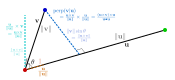
\includegraphics[width = \textwidth]{perp_by_cross_product}

\textbf{Examples:}
\begin{itemize}
\item Let \(\mathbf{u} = \begin{bmatrix} 6 \\ -2 \\ -8 \end{bmatrix}\) and \(\mathbf{v} = \begin{bmatrix} -1 \\ -1 \\ 6 \end{bmatrix}\). \\ 
\(\mathbf{u} \bullet \mathbf{u} = \|\mathbf{u}\|^2 = 6^2 + (-2)^2 + (-8)^2 = 36 + 4 + 64 = 104\), \\ 
\(\mathbf{u} \times \mathbf{v} = \begin{bmatrix} (-2)(6) - (-8)(-1) \\ (-8)(-1) - (6)(6) \\ (6)(-1) - (-2)(-1) \end{bmatrix} = \begin{bmatrix} -12 - 8 \\ 8 - 36 \\ -6 - 2 \end{bmatrix} = \begin{bmatrix} -20 \\ -28 \\ -8 \end{bmatrix}\), \\
\(\left\|\mathbf{u} \times \mathbf{v}\right\| = \sqrt{(-20)^2 + (-28)^2 + (-8)^2} = \sqrt{1248} = 4\sqrt{78}\), \\
\(\|\mathbf{u}\| = \sqrt{104} = 2\sqrt{26}\), \\
Therefore: \[\left\|\text{perp}(\mathbf{v} | \mathbf{u})\right\| = \frac{\left\|\mathbf{u} \times \mathbf{v}\right\|}{\|\mathbf{u}\|} = \frac{4\sqrt{78}}{2\sqrt{26}} = 2\sqrt{3}\] 
\((\mathbf{u} \times \mathbf{v}) \times \mathbf{u} = \begin{bmatrix} (-28)(-8) - (-8)(-2) \\ (-8)(6) - (-20)(-8) \\ (-20)(-2) - (-28)(6) \end{bmatrix} = \begin{bmatrix} 208 \\ -208 \\ 208 \end{bmatrix}\), \\
Therefore: \[\text{perp}(\mathbf{v} | \mathbf{u}) = \frac{(\mathbf{u} \times \mathbf{v}) \times \mathbf{u}}{\mathbf{u} \bullet \mathbf{u}} = \begin{bmatrix} 2 \\ -2 \\ 2 \end{bmatrix}\]
\end{itemize}




\section*{The scalar triple product}

Given a rectangular prism with a width of \(u\), a depth of \(v\), and a height of \(w\), the volume is \(V = u \cdot v \cdot w\). Now let \(\mathbf{u}\), \(\mathbf{v}\), and \(\mathbf{w}\) denote displacement vectors. Extruding the parallelogram that results from the cross product of \(\mathbf{u}\) and \(\mathbf{v}\) along the displacement \(\mathbf{w}\) results in a {\bf parallelepiped}, as depicted in the image below. The volume of this parallelepiped can be derived by first computing the surface vector of the parallelogram that results from the cross product of \(\mathbf{u}\) and \(\mathbf{v}\): \(\mathbf{A} = \mathbf{u} \times \mathbf{v}\). When this parallelogram is extruded along the displacement \(\mathbf{w}\), the volume becomes:
\[V = \mathbf{A} \bullet \mathbf{w} = (\mathbf{u} \times \mathbf{v}) \bullet \mathbf{w}\] 
This is referred to as the {\bf scalar triple product}. 

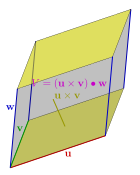
\includegraphics[width = 0.5\textwidth]{scalar_triple_product}

If \(\mathbf{w}\) points in a direction opposite \(\mathbf{A} = \mathbf{u} \times \mathbf{v}\), then the volume will be negative. The actual volume is in fact the absolute value of the scalar triple product:
\[V = \left|(\mathbf{u} \times \mathbf{v}) \bullet \mathbf{w}\right|\]  
The so called ``signed volume" of the scalar triple product \((\mathbf{u} \times \mathbf{v}) \bullet \mathbf{w}\) is useful in other cases.

It should also be noted that the ordering of \(\mathbf{u}\), \(\mathbf{v}\), and \(\mathbf{w}\) has no impact on the absolute value of the scalar triple product:
\[\left|(\mathbf{u} \times \mathbf{v}) \bullet \mathbf{w}\right| = \left|(\mathbf{u} \times \mathbf{w}) \bullet \mathbf{v}\right| = \left|(\mathbf{v} \times \mathbf{u}) \bullet \mathbf{w}\right|= \left|(\mathbf{v} \times \mathbf{w}) \bullet \mathbf{u}\right| = \left|(\mathbf{w} \times \mathbf{u}) \bullet \mathbf{v}\right| = \left|(\mathbf{w} \times \mathbf{v}) \bullet \mathbf{u}\right|\]

A single swap of 2 of the vectors \(\mathbf{u}\), \(\mathbf{v}\), and \(\mathbf{w}\) flips the sign of the scalar triple product:
\[(\mathbf{u} \times \mathbf{v}) \bullet \mathbf{w} = -(\mathbf{v} \times \mathbf{u}) \bullet \mathbf{w} = -(\mathbf{w} \times \mathbf{v}) \bullet \mathbf{u} = -(\mathbf{u} \times \mathbf{w}) \bullet \mathbf{v}\] 
while two swaps preserves the sign of the scalar triple product:
\[(\mathbf{u} \times \mathbf{v}) \bullet \mathbf{w} = (\mathbf{v} \times \mathbf{w}) \bullet \mathbf{u} = (\mathbf{w} \times \mathbf{u}) \bullet \mathbf{v}\]


\textbf{Examples:}
\begin{itemize}
%%%%%%%%%%%%%%%%%%%%%%
\item If \(\mathbf{u} = \begin{bmatrix} 3 \\ -1 \\ 2 \end{bmatrix}\), \(\mathbf{v} = \begin{bmatrix} 4 \\ 2 \\ -1 \end{bmatrix}\) and \(\mathbf{w} = \begin{bmatrix} -2 \\ -1 \\ 1 \end{bmatrix}\), then
\[\mathbf{u} \times \mathbf{v} = \begin{bmatrix} (-1)(-1) - (2)(2) \\ (2)(4) - (3)(-1) \\ (3)(2) - (-1)(4) \end{bmatrix} = \begin{bmatrix} 1 - 4 \\ 8 + 3 \\ 6 + 4 \end{bmatrix} = \begin{bmatrix} -3 \\ 11 \\ 10 \end{bmatrix}\]
\[(\mathbf{u} \times \mathbf{v}) \bullet \mathbf{w} = \begin{bmatrix} -3 \\ 11 \\ 10 \end{bmatrix} \bullet \begin{bmatrix} -2 \\ -1 \\ 1 \end{bmatrix} = (-3)(-2) + (11)(-1) + (10)(1) = 6 - 11 + 10 = 5\]
The volume of the parallelepiped bounded by \(\mathbf{u}\), \(\mathbf{v}\), and \(\mathbf{w}\) is \(V = (\mathbf{u} \times \mathbf{v}) \bullet \mathbf{w} = 5\).
%%%%%%%%%%%%%%%%%%%%%%
\item If \(\mathbf{u} = \begin{bmatrix} 4 \\ -1 \\ -3 \end{bmatrix}\), \(\mathbf{v} = \begin{bmatrix} 5 \\ -2 \\ -1 \end{bmatrix}\), and \(\mathbf{w} = \begin{bmatrix} 3 \\ -2 \\ 7 \end{bmatrix}\), then
\[\mathbf{u} \times \mathbf{v} = \begin{bmatrix} (-1)(-1) - (-3)(-2) \\ (-3)(5) - (4)(-1) \\ (4)(-2) - (-1)(5) \end{bmatrix} = \begin{bmatrix} 1 - 6 \\ -15 + 4 \\ -8 + 5 \end{bmatrix} = \begin{bmatrix} -5 \\ -11 \\ -3 \end{bmatrix}\]
\[(\mathbf{u} \times \mathbf{v}) \bullet \mathbf{w} = \begin{bmatrix} -5 \\ -11 \\ -3 \end{bmatrix} \bullet \begin{bmatrix} 3 \\ -2 \\7 \end{bmatrix} = (-5)(3) + (-11)(-2) + (-3)(7) = -15 + 22 - 21 = -14\]
The volume of the parallelepiped bounded by \(\mathbf{u}\), \(\mathbf{v}\), and \(\mathbf{w}\) is \(V = |(\mathbf{u} \times \mathbf{v}) \bullet \mathbf{w}| = 14\).
\end{itemize}




\section*{Examples:}

%%%%%%%%%%%%%%%%%%%%%%%%%%%%%%%%%%%%%%%%
%%%%%%%%%%%%%%%%%%%%%%%%%%%%%%%%%%%%%%%%
\subsection*{Example 1:}

Let \(\mathbf{u} = \begin{bmatrix} 2 \\ -5 \\ 7 \end{bmatrix}\) and \(\mathbf{v} = \begin{bmatrix} 1 \\ 9 \\ -4 \end{bmatrix}\):
\begin{itemize}
%%%%%%%%%%%%%%%%%%%
\item[*] \begin{align*}
\mathbf{u} + \mathbf{v} = & \begin{bmatrix} 2 \\ -5 \\ 7 \end{bmatrix} + \begin{bmatrix} 1 \\ 9 \\ -4 \end{bmatrix} 
= \begin{bmatrix} 2 + 1 \\ (-5) + 9 \\ 7 + (-4) \end{bmatrix} = \begin{bmatrix} 3 \\ 4 \\ 3 \end{bmatrix}
\end{align*}
%%%%%%%%%%%%%%%%%%%
\item[*] \begin{align*}
\mathbf{u} - \mathbf{v} = & \begin{bmatrix} 2 \\ -5 \\ 7 \end{bmatrix} - \begin{bmatrix} 1 \\ 9 \\ -4 \end{bmatrix} 
= \begin{bmatrix} 2 - 1 \\ (-5) - 9 \\ 7 - (-4) \end{bmatrix} = \begin{bmatrix} 1 \\ -14 \\ 11 \end{bmatrix}
\end{align*}
%%%%%%%%%%%%%%%%%%%
\item[*] \begin{align*}
2\mathbf{u} = & 2 \begin{bmatrix} 2 \\ -5 \\ 7 \end{bmatrix} = \begin{bmatrix} (2)(2) \\ (2)(-5) \\ (2)(7) \end{bmatrix} = \begin{bmatrix} 4 \\ -10 \\ 14 \end{bmatrix}
\end{align*}    
%%%%%%%%%%%%%%%%%%%
\item[*] \begin{align*}
-3\mathbf{u} + 5\mathbf{v} = & -3\begin{bmatrix} 2 \\ -5 \\ 7 \end{bmatrix} + 5\begin{bmatrix} 1 \\ 9 \\ -4 \end{bmatrix} 
= \begin{bmatrix} -6 \\ 15 \\ -21 \end{bmatrix} + \begin{bmatrix} 5 \\ 45 \\ -20 \end{bmatrix}
= \begin{bmatrix} -1 \\ 60 \\ -41 \end{bmatrix} 
\end{align*}
%%%%%%%%%%%%%%%%%%%
\item[*] \begin{align*}
9\mathbf{u} + 5\mathbf{v} = & 9\begin{bmatrix} 2 \\ -5 \\ 7 \end{bmatrix} + 5\begin{bmatrix} 1 \\ 9 \\ -4 \end{bmatrix} 
= \begin{bmatrix} 18 \\ -45 \\ 63 \end{bmatrix} + \begin{bmatrix} 5 \\ 45 \\ -20 \end{bmatrix} 
= \begin{bmatrix} 23 \\ 0 \\ 43 \end{bmatrix}  
\end{align*}
%%%%%%%%%%%%%%%%%%%
\item[*] \begin{align*}
\left\|\mathbf{u}\right\| = & \left\|\begin{bmatrix} 2 \\ -5 \\ 7 \end{bmatrix}\right\|  
= \sqrt{2^2 + (-5)^2 + 7^2} 
= \sqrt{4 + 25 + 49} 
= \sqrt{78}
\end{align*}
%%%%%%%%%%%%%%%%%%%
\item[*] \begin{align*}
\frac{\mathbf{u}}{\left\|\mathbf{u}\right\|} = & \frac{1}{\sqrt{78}}\begin{bmatrix} 2 \\ -5 \\ 7 \end{bmatrix}  
= \begin{bmatrix} 2/\sqrt{78} \\ -5/\sqrt{78} \\ 7/\sqrt{78} \end{bmatrix}
\end{align*}
%%%%%%%%%%%%%%%%%%%
\item[*] \begin{align*}
\left\|\mathbf{v}\right\| = & \left\|\begin{bmatrix} 1 \\ 9 \\ -4 \end{bmatrix}\right\|  
= \sqrt{1^2 + 9^2 + (-4)^2} 
= \sqrt{1 + 81 + 16} 
= \sqrt{98}
\end{align*}
%%%%%%%%%%%%%%%%%%%
\item[*] \begin{align*}
\frac{\mathbf{v}}{\left\|\mathbf{v}\right\|} = & \frac{1}{\sqrt{98}}\begin{bmatrix} 1 \\ 9 \\ -4 \end{bmatrix}  
= \begin{bmatrix} 1/\sqrt{98} \\ 9/\sqrt{98} \\ -4/\sqrt{98} \end{bmatrix}
\end{align*}
%%%%%%%%%%%%%%%%%%%
\item[*] \begin{align*}
\mathbf{u} \bullet \mathbf{v} = & \begin{bmatrix} 2 \\ -5 \\ 7 \end{bmatrix} \bullet \begin{bmatrix} 1 \\ 9 \\ -4 \end{bmatrix} 
= (2)(1) + (-5)(9) + (7)(-4) 
= 2 - 45 - 28 
= -71
\end{align*}
%%%%%%%%%%%%%%%%%%%
\item[*] \begin{align*}
\text{proj}(\mathbf{v} | \mathbf{u}) = & \frac{\mathbf{u} \bullet \mathbf{v}}{\mathbf{u} \bullet \mathbf{u}}\mathbf{u}
= \frac{-71}{78}\begin{bmatrix} 2 \\ -5 \\ 7 \end{bmatrix} 
= \begin{bmatrix} -71/39 \\ 355/78 \\ -497/78 \end{bmatrix}
\end{align*}
%%%%%%%%%%%%%%%%%%%
\item[*] \begin{align*}
\text{perp}(\mathbf{v} | \mathbf{u}) = & \mathbf{v} - \text{proj}(\mathbf{v} | \mathbf{u})
= \begin{bmatrix} 1 \\ 9 \\ -4 \end{bmatrix} - \begin{bmatrix} -71/39 \\ 355/78 \\ -497/78 \end{bmatrix} 
= \begin{bmatrix} 110/39 \\ 347/78 \\ 185/78 \end{bmatrix}
\end{align*}
%%%%%%%%%%%%%%%%%%%
\item[*] \begin{align*}
\theta = & \cos^{-1}\left(\frac{\mathbf{u} \bullet \mathbf{v}}{\left\|\mathbf{u}\right\| \left\|\mathbf{v}\right\|}\right)  
= \cos^{-1}\left(\frac{-71}{\sqrt{78} \cdot \sqrt{98}}\right) 
= \cos^{-1}\left(\frac{-71}{14\sqrt{39}}\right)   
\approx 144.300^\circ
\end{align*}  
%%%%%%%%%%%%%%%%%%%
\item[*] \begin{align*}
\mathbf{u} \times \mathbf{v} = & \begin{bmatrix} 2 \\ -5 \\ 7 \end{bmatrix} \times \begin{bmatrix} 1 \\ 9 \\ -4 \end{bmatrix}  
= \begin{bmatrix} (-5)(-4) - (7)(9) \\ (7)(1) - (2)(-4) \\ (2)(9) - (-5)(1) \end{bmatrix} 
= \begin{bmatrix} 20 - 63 \\ 7 - (-8) \\ 18 - (-5) \end{bmatrix} 
= \begin{bmatrix} -43 \\ 15 \\ 23 \end{bmatrix}
\end{align*}
\end{itemize}


%%%%%%%%%%%%%%%%%%%%%%%%%%%%%%%%%%%%%%%%
%%%%%%%%%%%%%%%%%%%%%%%%%%%%%%%%%%%%%%%%
\subsection*{Example 2:}

Let \(\mathbf{u} = \begin{bmatrix} 1 \\ 2 \\ 3 \end{bmatrix}\) and \(\mathbf{v} = \begin{bmatrix} 3 \\ 2 \\ 1 \end{bmatrix}\):
\begin{itemize}
%%%%%%%%%%%%%%%%%%%
\item[*] \begin{align*}
\left\|\mathbf{u}\right\| = & \left\|\begin{bmatrix} 1 \\ 2 \\ 3 \end{bmatrix}\right\|  
= \sqrt{1^2 + 2^2 + 3^2} 
= \sqrt{1 + 4 + 9} 
= \sqrt{14}
\end{align*}
%%%%%%%%%%%%%%%%%%%
\item[*] \begin{align*}
\frac{\mathbf{u}}{\left\|\mathbf{u}\right\|} = & \frac{1}{\sqrt{14}}\begin{bmatrix} 1 \\ 2 \\ 3 \end{bmatrix} 
= \begin{bmatrix} 1/\sqrt{14} \\ 2/\sqrt{14} \\ 3/\sqrt{14} \end{bmatrix}
\end{align*}
%%%%%%%%%%%%%%%%%%%
\item[*] \begin{align*}
\left\|\mathbf{v}\right\| = & \left\|\begin{bmatrix} 3 \\ 2 \\ 1 \end{bmatrix}\right\|  
= \sqrt{3^2 + 2^2 + 1^2} 
= \sqrt{9 + 4 + 1} 
= \sqrt{14}
\end{align*}
%%%%%%%%%%%%%%%%%%%
\item[*] \begin{align*}
\frac{\mathbf{v}}{\left\|\mathbf{v}\right\|} = & \frac{1}{\sqrt{14}}\begin{bmatrix} 3 \\ 2 \\ 1 \end{bmatrix} 
= \begin{bmatrix} 3/\sqrt{14} \\ 2/\sqrt{14} \\ 1/\sqrt{14} \end{bmatrix}
\end{align*}
%%%%%%%%%%%%%%%%%%%
\item[*] \begin{align*}
\mathbf{u} \bullet \mathbf{v} = & \begin{bmatrix} 1 \\ 2 \\ 3 \end{bmatrix} \bullet \begin{bmatrix} 3 \\ 2 \\ 1 \end{bmatrix} 
= (1)(3) + (2)(2) + (3)(1) 
= 3 + 4 + 3
= 10  
\end{align*}
%%%%%%%%%%%%%%%%%%%
\item[*] \begin{align*}
\text{proj}(\mathbf{v} | \mathbf{u}) = & \frac{\mathbf{u} \bullet \mathbf{v}}{\mathbf{u} \bullet \mathbf{u}}\mathbf{u}
= \frac{10}{14}\begin{bmatrix} 1 \\ 2 \\ 3 \end{bmatrix} 
= \begin{bmatrix} 5/7 \\ 10/7 \\ 15/7 \end{bmatrix}
\end{align*}
%%%%%%%%%%%%%%%%%%%
\item[*] \begin{align*}
\text{perp}(\mathbf{v} | \mathbf{u}) = & \mathbf{v} - \text{proj}(\mathbf{v} | \mathbf{u})
= \begin{bmatrix} 3 \\ 2 \\ 1 \end{bmatrix} - \begin{bmatrix} 5/7 \\ 10/7 \\ 15/7 \end{bmatrix} 
= \begin{bmatrix} 16/7 \\ 4/7 \\ -8/7 \end{bmatrix}
\end{align*}
%%%%%%%%%%%%%%%%%%%
\item[*] \begin{align*}
\theta = & \cos^{-1}\left(\frac{\mathbf{u} \bullet \mathbf{v}}{\left\|\mathbf{u}\right\| \left\|\mathbf{v}\right\|}\right)  
= \cos^{-1}\left(\frac{10}{\sqrt{14} \cdot \sqrt{14}}\right) 
= \cos^{-1}\left(\frac{5}{7}\right)   
\approx 44.4153^\circ
\end{align*}  
%%%%%%%%%%%%%%%%%%%
\item[*] \begin{align*}
\mathbf{u} \times \mathbf{v} = & \begin{bmatrix} 1 \\ 2 \\ 3 \end{bmatrix} \times \begin{bmatrix} 3 \\ 2 \\ 1 \end{bmatrix}  
= \begin{bmatrix} (2)(1) - (3)(2) \\ (3)(3) - (1)(1) \\ (1)(2) - (2)(3) \end{bmatrix} 
= \begin{bmatrix} 2 - 6 \\ 9 - 1 \\ 2 - 6 \end{bmatrix} 
= \begin{bmatrix} -4 \\ 8 \\ -4 \end{bmatrix}
\end{align*}
%%%%%%%%%%%%%%%%%%%
\item[*] \begin{align*}
\left\|\mathbf{u} \times \mathbf{v}\right\| = & \left\|\begin{bmatrix} -4 \\ 8 \\ -4 \end{bmatrix}\right\|  
= \sqrt{(-4)^2 + 8^2 + (-4)^2} 
= \sqrt{16 + 64 + 16} 
= \sqrt{96} 
= 4\sqrt{6}
\end{align*}
%%%%%%%%%%%%%%%%%%%
\item[*] \begin{align*}
\sin\theta = & \frac{\left\|\mathbf{u} \times \mathbf{v}\right\|}{\left\|\mathbf{u}\right\| \left\|\mathbf{v}\right\|} 
= \frac{4\sqrt{6}}{\sqrt{14} \cdot \sqrt{14}} 
= \frac{2\sqrt{6}}{7} 
\end{align*}
%%%%%%%%%%%%%%%%%%%
\item[*] \begin{align*}
\cos^2\theta + \sin^2\theta 
= & \left(\frac{5}{7}\right)^2 + \left(\frac{2\sqrt{6}}{7}\right)^2 
= \frac{25}{49} + \frac{24}{49} = 1
\end{align*}
\end{itemize}




%%%%%%%%%%%%%%%%%%%%%%%%%%%%%%%%%%%%%%%%
%%%%%%%%%%%%%%%%%%%%%%%%%%%%%%%%%%%%%%%%
\subsection*{Example 3:}

Let the points \(P\), \(Q\), and \(R\) be:
\[P(-1, 2, 3) \quad\text{and}\quad Q(2, 1, 2) \quad\text{and}\quad R(5, -1, -1)\] 
\begin{itemize}
%%%%%%%%%%%%%%%%%%%
\item[*] \begin{align*}
\overrightarrow{PQ} = & \begin{bmatrix} 2 - (-1) \\ 1 - 2 \\ 2 - 3 \end{bmatrix} = \begin{bmatrix} 3 \\ -1 \\ -1 \end{bmatrix}
\end{align*}
%%%%%%%%%%%%%%%%%%%
\item[*] The distance between points \(P\) and \(Q\) is: 
\[PQ = \left\|\overrightarrow{PQ}\right\| = \sqrt{3^2 + (-1)^2 + (-1)^2} = \sqrt{9 + 1 + 1} = \sqrt{11} \approx 3.31662\]
%%%%%%%%%%%%%%%%%%%
\item[*] \begin{align*}
\overrightarrow{PR} = & \begin{bmatrix} 5 - (-1) \\ (-1) - 2 \\ (-1) - 3 \end{bmatrix} = \begin{bmatrix} 6 \\ -3 \\ -4 \end{bmatrix}
\end{align*}
%%%%%%%%%%%%%%%%%%%
\item[*] \begin{align*}
\overrightarrow{PQ} \times \overrightarrow{PR} = & \begin{bmatrix} (-1)(-4) - (-1)(-3) \\ (-1)(6) - (3)(-4) \\ (3)(-3) - (-1)(6) \end{bmatrix} = \begin{bmatrix} 4 - 3 \\ -6 + 12 \\ -9 + 6 \end{bmatrix} = \begin{bmatrix} 1 \\ 6 \\ -3 \end{bmatrix}
\end{align*}
%%%%%%%%%%%%%%%%%%%
\item[*] The triangle \(\Delta PQR\) has an area of:   
\begin{align*}
A = & \frac{1}{2}\left\|\overrightarrow{PQ} \times \overrightarrow{PR}\right\|  
= \frac{1}{2}\left\|\begin{bmatrix} 1 \\ 6 \\ -3 \end{bmatrix}\right\| 
= \frac{1}{2}\sqrt{1^2 + 6^2 + (-3)^2} 
= \frac{1}{2}\sqrt{1 + 36 + 9} = \frac{1}{2}\sqrt{46} \approx 3.39116
\end{align*}
\end{itemize}




%%%%%%%%%%%%%%%%%%%%%%%%%%%%%%%%%%%%%%%%
%%%%%%%%%%%%%%%%%%%%%%%%%%%%%%%%%%%%%%%%

\subsection*{Example 4:}

Let the points \(P\), \(Q\), and \(R\) be:
\[P(5, 3, 1) \quad\text{and}\quad Q(6, 5, 2) \quad\text{and}\quad R(-1, 2, 4)\]
\begin{itemize}
%%%%%%%%%%%%%%%%%%%
\item[*] \begin{align*}
\overrightarrow{PQ} = & \begin{bmatrix} 6 - 5 \\ 5 - 3 \\ 2 - 1 \end{bmatrix} = \begin{bmatrix} 1 \\ 2 \\ 1 \end{bmatrix}
\end{align*}
%%%%%%%%%%%%%%%%%%%
\item[*] The distance between points \(P\) and \(Q\) is: 
\[PQ = \left\|\overrightarrow{PQ}\right\| = \sqrt{1^2 + 2^2 + 1^2} = \sqrt{1 + 4 + 1} = \sqrt{6} \approx 2.44949\]
%%%%%%%%%%%%%%%%%%%
\item[*] \begin{align*}
\overrightarrow{PR} = & \begin{bmatrix} (-1) - 5 \\ 2 - 3 \\ 4 - 1 \end{bmatrix} = \begin{bmatrix} -6 \\ -1 \\ 3 \end{bmatrix}
\end{align*}
%%%%%%%%%%%%%%%%%%%
\item[*] \begin{align*}
\overrightarrow{PQ} \times \overrightarrow{PR} = & \begin{bmatrix} (2)(3) - (1)(-1) \\ (1)(-6) - (1)(3) \\ (1)(-1) - (2)(-6) \end{bmatrix} = \begin{bmatrix} 6 + 1 \\ -6 - 3 \\ -1 + 12 \end{bmatrix} = \begin{bmatrix} 7 \\ -9 \\ 11 \end{bmatrix}
\end{align*}
%%%%%%%%%%%%%%%%%%%
\item[*] The triangle \(\Delta PQR\) has an area of:   
\begin{align*}
A = & \frac{1}{2}\left\|\overrightarrow{PQ} \times \overrightarrow{PR}\right\|  
= \frac{1}{2}\left\|\begin{bmatrix} 7 \\ -9 \\ 11 \end{bmatrix} \right\| 
= \frac{1}{2}\sqrt{7^2 + (-9)^2 + 11^2} 
= \frac{1}{2}\sqrt{49 + 81 + 121} = \frac{1}{2}\sqrt{251} \approx 7.92149
\end{align*}
\end{itemize}


\end{document}





